\chapter{基于神经网络的生成模型}
\label{chap:neural-generative-models}

先做一个角色上的对比。前面各章的网络基本都在做“判别”或“预测”：给定一张手写数字图像，分类网络输出它是0到9中的哪一个——对每一个输入，都存在一个由数据集明确规定的正确答案。现在把问题整个反过来：只给你一大批手写数字，不指定任何具体答案，请你凭空造出一张这堆数据里不曾出现、但看上去同样真实的新图像。这就是生成任务。输出不再是某张已有图像的类别，而是一个全新的观测；训练数据只告诉我们“哪些图像曾经出现、大致长什么样”，却没有为你这一次生成指定唯一正确的像素值。

这种“没有标准答案”正是生成模型困难和有趣的根源。用本章一个具体例子可以说清难处：如果网络只会输出一张固定图像，那么使平均像素平方误差最小的那张图，其实是所有训练图的平均值——不同位置、不同写法的笔画叠加在一起，只会得到一团模糊的灰影。哪怕生成器能输出很多张图，但若它翻来覆去只会画一种最清楚的“3”，它依然没有还原数据中数字0到9以及同一数字千变万化的写法。空白图、单一输出、死记硬背几张训练图，都不合格。因此生成模型必须同时做到两件事，本章会反复回到这两条标准：一是每张生成图本身要合理（像真实数据），二是所有生成图合起来要覆盖真实数据的全部变化范围（分布对得上），后者尤其容易被忽视。

前面学过的网络构件仍然有用：卷积网络可以把小尺寸特征逐步放大成图像，前馈网络可以把随机输入变换成连续向量。本章沿“用一个网络产生样本，再用另一个网络评判样本”这条对抗学习的主线展开：对抗目标提供共同的学习信号，卷积结构改善图像的空间组织；当来源分类无法反映两组观测正在逐渐接近时，需要换一种分布比较方式（WGAN）；条件信息和来回重建支持受控生成与图像转换；分层调节则把控制权放进图像生成的不同尺度。至于通过显式似然、潜变量后验推断、可逆密度变换，或逐步加噪再去噪的扩散过程来学习的另一大类生成模型，见\BookChapterRef{chap:pgm-generative}{卷6《模型：概率图模型》的“概率生成模型”章}。本章的网络同样规定了一个概率分布，区别在于主要通过采样和判别来学习并使用这个分布。

\section{生成任务与采样网络}
\label{sec:neural-generative-task}

\subsection{从预测一个结果到生成一组可能观测}
\label{sec:neural-generative-observations}

一批手写数字既包含不同数字，也包含同一数字的不同写法。即使指定生成数字“3”，笔画粗细、倾斜方向和弯曲程度也可以不同。生成模型需要保留这些可能性，因此不能只用一个固定向量代表全部输出，而应当描述“输出在各种可能图像上的概率分布”。

记观测空间为$\bm{S}\subseteq\mathbb{R}^{d}$，真实观测的分布为$P$，训练样本为独立同分布的$\bm{x}_1,\ldots,\bm{x}_n\sim P$。对一张$28\times28$的灰度图，$d=784$，一个观测包含全部像素。模型生成的分布记为$Q_{\bm{\theta}}$；学习的目标是让它在所选择的比较准则下逼近$P$，而不只是使个别输出看起来合理。请特别注意这里目标的层次：监督学习是让单个输出$G(\bm{x})$逼近单个标签$y$，生成学习却是让一整个分布$Q_{\bm{\theta}}$逼近另一个分布$P$，评价对象是“两堆样本的规律是否相同”，这也是后续必须引入判别器等专门工具的根本原因。

如果直接把每张训练图都与同一个输出比较，再最小化像素平方误差，最优固定输出就是训练图的平均值。可以用一个直观的概率论证理解：要最小化$\mathbb{E}\lVert \bm{X}-\bm{c}\rVert^2$，最佳的固定$\bm{c}$正是$\mathbb{E}\bm{X}$。不同位置的笔画叠在一起，容易得到一张模糊图。这种目标适合估计平均像素，却没有要求输出分别覆盖不同写法。对没有一一配对关系的生成样本，先任意配上一张训练图再做像素回归，同样会把任意配对带来的差异当作误差。

生成的评价因而需要比较两组观测的规律。例如，在一维教学例子中，真实数据一半集中在$-2$附近，另一半集中在$2$附近。模型只生成右侧一团时，输出所在位置可以合理，但左侧出现的可能性已经丢失；若每次都固定输出总体均值$0$，则连两团数据的位置都没有保留。

为了用密度曲线显示这种位置偏离，图~\ref{fig:neural-generative-modes}在左侧另行构造了一个只在均值$0$附近生成的单峰分布。它允许输出在$0$附近变化，仍没有覆盖两侧的真实数据团。固定均值的例子每次输出同一个点，图中的单峰候选则具有图注给定的非零方差；两者承担同一个位置偏离的说明任务，随机性不同。右图再用只覆盖右侧的候选，说明输出位置合理仍可能遗漏另一团。图中两个候选由此分别展示位置拟合与覆盖范围的问题。
\begin{figure*}[htbp]
  \centering
  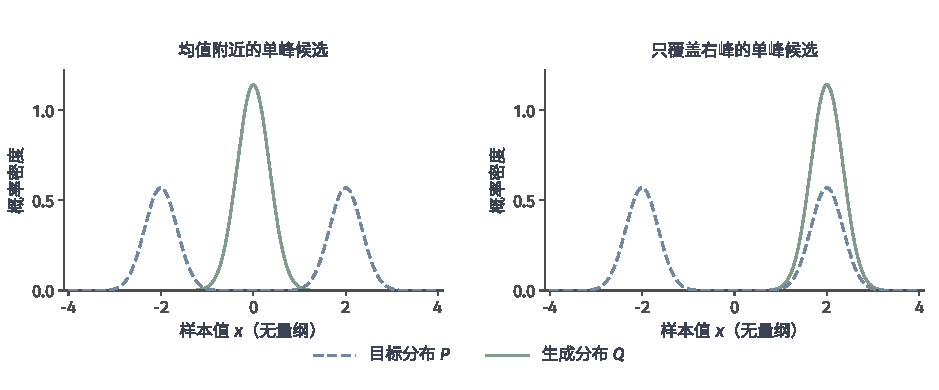
\includegraphics[width=159mm]{figures/08-neural-network-models/00-shared/matplotlib/neural-generative-objectives/modes/figure.pdf}
  \caption{两种生成分布与同一个双峰目标比较。目标为等权重的$\mathcal{N}(-2,0.35^2)$和$\mathcal{N}(2,0.35^2)$混合；左图的生成分布为$\mathcal{N}(0,0.35^2)$，右图为$\mathcal{N}(2,0.35^2)$。虚线目标在两侧各有一半概率，实线分别显示生成平均位置与只覆盖一侧的差异。曲线由给定密度精确计算，不是训练实验。}
  \label{fig:neural-generative-modes}
\end{figure*}

\subsection{随机输入与生成器}
\label{sec:neural-generative-sampling}

要让一个确定性的网络每次产生不同的输出，就得给它喂入一个每次都不同的输入。最方便的随机源是一个容易采样的简单分布（如标准高斯），让网络学会把这些简单随机数“塑造”成符合数据规律的复杂样本——这很像把一团均匀的黏土塑造成各种手型，网络参数决定塑形的规则。令$\bm{Z}\in\mathbb{R}^{k}$服从固定分布$\nu$，例如标准高斯或均匀分布；带参数的网络$G_{\bm{\theta}}:\mathbb{R}^{k}\to\bm{S}$产生
\begin{equation}
  \label{eq:neural-generative-sample}
  \widetilde{\bm{X}}=G_{\bm{\theta}}(\bm{Z}),\qquad \bm{Z}\sim\nu.
\end{equation}
这个网络称为\term{生成器}（generator）。随机输入负责提供变化，网络负责把变化组织成符合数据规律的观测。固定$\bm{\theta}$后，每抽取一个新的$\bm{Z}$就得到一个新的样本；但要强调，加入随机向量只是给了多样性的“可能”，并不自动保证多样——如果网络对所有$\bm{Z}$都输出几乎相同的图，随机输入就被它忽略了，这正是后面要靠训练目标去防止的模式坍缩。

式~\eqref{eq:neural-generative-sample}已经确定生成分布。这里要引入一个初学者很容易忽略的区分：我们能从网络“抽样”，却通常无法对任意一张给定图像直接写出它的概率密度。对任意可测观测集合$A\subseteq\bm{S}$，
\begin{equation}
  \label{eq:neural-generative-distribution}
  Q_{\bm{\theta}}(A)=\mathbb{P}_{\bm{Z}\sim\nu}
    \{G_{\bm{\theta}}(\bm{Z})\in A\}.
\end{equation}
例如，“生成的图像中出现闭合圆圈”对应一个图像集合；这个集合在$Q_{\bm{\theta}}$下的概率，由多少随机输入被映射到该集合决定。能从网络抽样，不意味着能直接算出某张图像的密度——求密度相当于追问“有哪些、有多少$\bm Z$被映到了这张图附近”，在高维非线性网络下极难计算。这类主要由采样程序隐式给出分布、却不直接给出密度表达式的模型，称为\term{隐式生成模型}（implicit generative model），GAN正是其中代表，这也解释了它为什么不能像分类那样直接拿“真实密度”作损失，而要另辟蹊径。

记$\bm{\Theta}$为允许的参数集合，生成器的候选空间为$\{G_{\bm{\theta}}:\bm{\theta}\in\bm{\Theta}\}$，对应的候选分布为$\{Q_{\bm{\theta}}:\bm{\theta}\in\bm{\Theta}\}$。网络宽度、深度、连接和输出范围共同限制这些候选。对于灰度图，可以在输出层用sigmoid把像素限制在$[0,1]$，也可以先把数据缩放到$[-1,1]$再使用tanh。输入维数$k$控制随机源的坐标数，但不能直接等同于可表达的类别数或视觉因素数。

\section{生成对抗网络}
\label{sec:neural-generative-gan}

\subsection{网络结构}
\label{sec:neural-generative-gan-structure}

生成器能产生一批图像了，但马上遇到一个棘手问题：没有真实图像能和它的输出逐像素配对，那损失该怎么定义？怎样告诉生成器“这张假图哪里不好、该往哪个方向改”？GAN给出了一个极巧妙的答案——利用一个天然存在、无需人工标注的标签：每张图要么“来自真实数据集”，要么“来自生成器”。既然如此，就可以再训练一个二分类网络专门区分这两种来源，并让生成器努力生成让它分不清的图。可以训练一个二分类网络来区分这两种来源，再让生成器朝着更难被区分的方向调整。

例如，生成的数字“3”缺少下半段弧线时，我们没有一张指定的真实图可逐像素对照，但真实训练图提供了完整笔画的例子。来源分类网络可以根据这些笔画差异降低生成图的评分。当评分对输入图像的梯度存在且非零时，沿梯度作足够小的改变就能提高当前图像的评分。生成器再把这个信号回传到参数，调整从随机输入产生图像的规则；它实际能作出的改变还受生成网络的结构限制。随后可以用新的一批输出检查差异。比较规则由训练中的网络学习，因而不必预先为每一种笔画错误手写一个评分函数。

Goodfellow等在2014年提出\term{生成对抗网络}（generative adversarial network, GAN），把这两个网络放入共同的学习过程。生成器$G_{\bm{\theta}}$产生样本，\term{判别器}（discriminator）$D_{\bm{\phi}}:\bm{S}\to(0,1)$估计在真实与生成来源等概率的训练设定下，一个输入来自真实数据的概率。$\bm{\theta}$和$\bm{\phi}$分别是两套待学习参数，判别器输出的“真实”是来源标签，不是图像内容的类别\scite{pgm-generative-goodfellow2014}

这两个网络承担不同的计算，理解它们的分工时可以把判别器想象成一位越来越挑剔的鉴画师，而生成器是拼命临摹以骗过鉴画师的造假者：鉴画师眼力越练越毒，造假者的手艺也被迫越来越高，理想终局是假画足以乱真、鉴画师只能靠猜（对每张图给出约$1/2$的真实概率）。一个教学性的全连接生成器可以把$k$维随机向量依次变成若干隐藏表示，最后输出$d$个像素；判别器则从$d$个像素提取特征，末层用sigmoid输出一个来源概率。生成器并非判别器的逆函数，两方也不共享待学习参数。生成器输出与判别器输入处于同一个观测空间，生成图可以直接送入判别器；判别器对图像的梯度便能沿生成路径继续回传，成为生成器的更新信号。GAN规定这套相互学习的方式，不规定隐藏层必须采用全连接结构。

真实图像送入判别器时标签为1，生成图像送入判别器时标签为0，两条路径使用同一套判别器参数。判别器希望两种来源可分，生成器希望自己的输出使来源更难分辨。图~\ref{fig:neural-generative-gan-structure}展开两方的内部层与共同输入路径；生成时只保留从随机输入到生成样本的生成器。
\begin{figure*}[htbp]
  \centering
  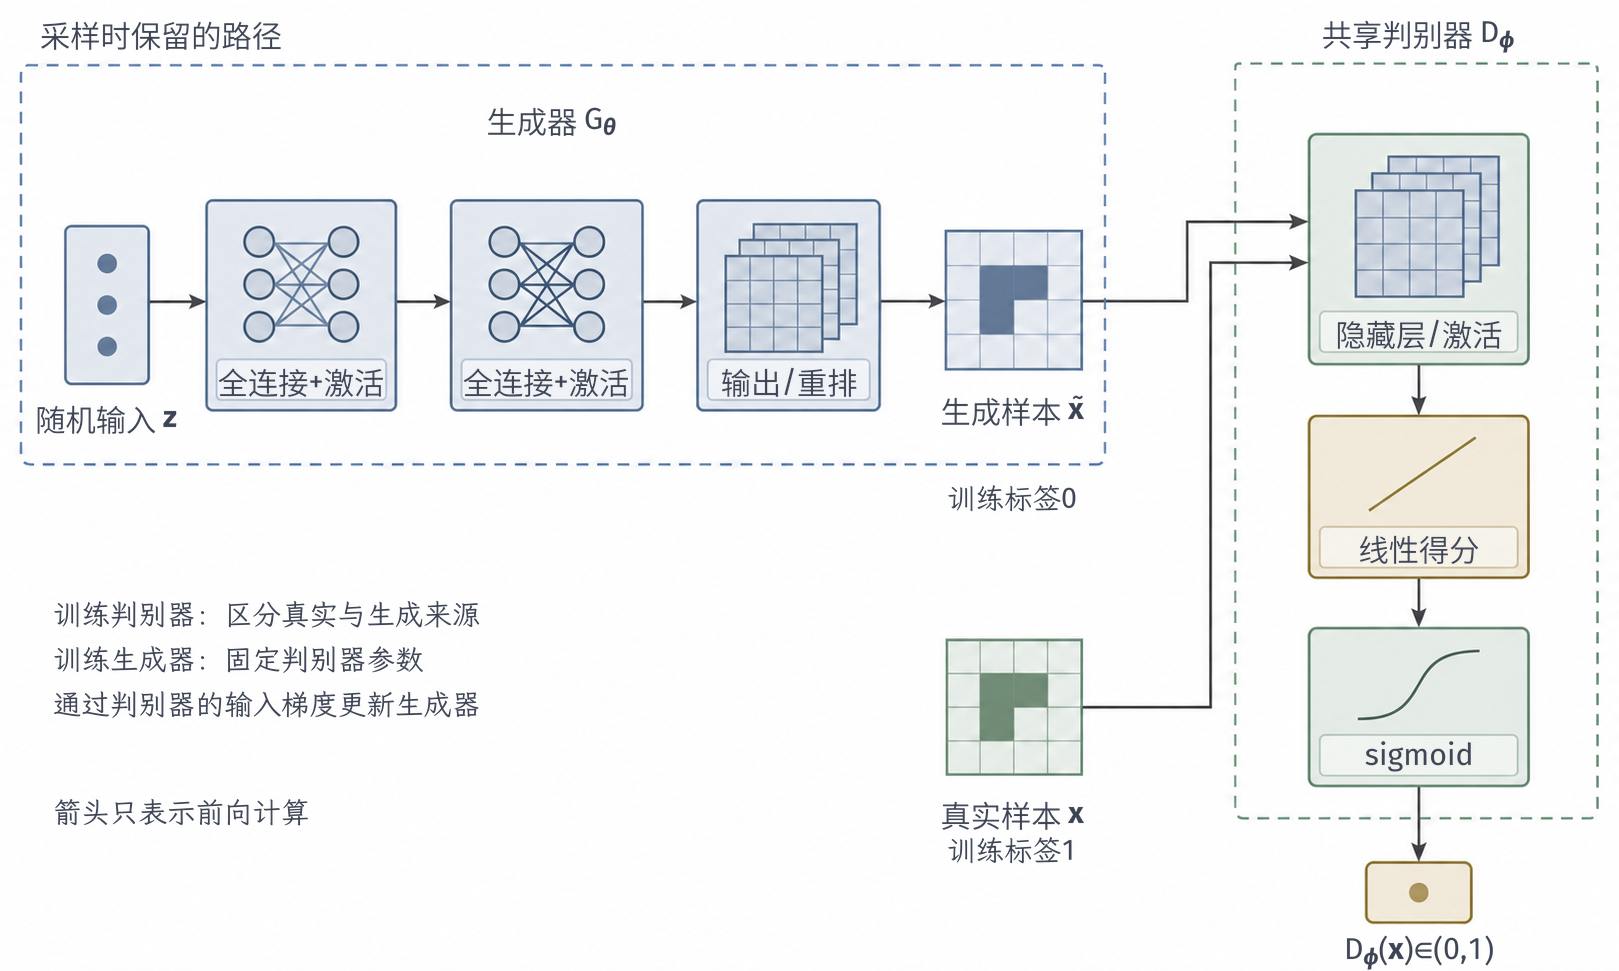
\includegraphics[width=150mm]{figures/08-neural-network-models/00-shared/generated/neural-generative-architectures/gan/figure.png}
  \caption{GAN的一种全连接结构。生成器逐层把随机输入映射为观测，真实与生成观测进入同一个判别器；单一得分经sigmoid变成来源概率。蓝色虚线区域是采样时保留的路径。来源标签用于训练判别器，不是其输入；更新生成器时固定判别器参数，并通过判别器对输入的导数回传梯度。箭头只表示前向计算。}
  \label{fig:neural-generative-gan-structure}
\end{figure*}

判别器不是一套预先固定的视觉规则。开始时，它可能只发现明显的像素范围或笔画差异；生成器改变后，判别器又根据新的样本寻找差异。这使生成器接收到随训练变化的比较信号，也使训练目标随另一方参数的变化而变化。

\subsection{参数学习}
\label{sec:neural-generative-gan-learning}

对两种来源使用二分类对数似然，判别器应增大真实样本的$\log D$和生成样本的$\log(1-D)$。记总体目标及其样本近似为
\begin{equation}
  \label{eq:neural-generative-gan-game}
  \begin{aligned}
  V(\bm{\theta},\bm{\phi})
    ={}&\mathbb{E}_{\bm{X}\sim P}\log D_{\bm{\phi}}(\bm{X})\\
      &+\mathbb{E}_{\bm{Z}\sim\nu}
         \log\{1-D_{\bm{\phi}}(G_{\bm{\theta}}(\bm{Z}))\},\\
  \widehat V(\bm{\theta},\bm{\phi})
    ={}&\frac1n\sum_{i=1}^{n}\log D_{\bm{\phi}}(\bm{x}_i)\\
      &+\frac1m\sum_{j=1}^{m}
         \log\{1-D_{\bm{\phi}}(G_{\bm{\theta}}(\bm{z}_j))\}.
  \end{aligned}
\end{equation}
这里$\bm{z}_1,\ldots,\bm{z}_m$独立取自$\nu$，与真实样本独立。原始GAN选择$\min_{\bm{\theta}}\max_{\bm{\phi}}V$：判别器尽量找到来源差异，生成器尽量减小可被找到的差异。真实项不含生成器参数，因此生成器只通过第二项更新。

实际训练交替固定一方、更新另一方。先抽取一批真实样本和随机输入，固定生成器，对$-\widehat V$做若干步梯度下降；再固定判别器，把生成样本经过判别器所得的梯度回传给生成器。固定判别器指不更新它的参数，仍需计算它对输入的导数。每轮通常重新抽取随机输入，真实数据则通过小批量读取；更新次数与步长决定两方变化的相对速度。

这与前面单个分类网络的学习有一处重要差别，也是理解GAN训练为何容易不稳定的关键。分类器的标签和损失规则通常已经固定，训练只是去逼近一个不变的目标；GAN中的一方每次改变参数，都会改变另一方正在面对的目标——这是一场没有固定靶子的博弈。判别器刚学会识别某种断裂笔画，生成器就可能修补这种笔画；生成器产生了新错误后，判别器又需要学习新的区分依据。对抗学习由此不断调整比较规则，也使“一方的损失下降”不能直接等同于整个生成任务持续改进。

博弈形式在数学上很优雅，但直接照它实现生成器更新会踩一个训练初期的坑，值得专门讨论。训练刚开始时生成器很差，产出的图一眼就能被识破，$D(G(\bm{z}))$可能很小。若判别器最后一层是sigmoid，记其生成样本得分为$a$，则$D=\sigma(a)$，此时让生成器去最小化“被判定为假”的损失$\log(1-D)$，其对得分的导数为
\[
  \frac{\mathrm{d}\log(1-\sigma(a))}{\mathrm{d}a}
    =-\sigma(a).
\]
当$a$远小于0、$D$接近0时，这个系数接近0——也就是说，恰恰在生成器最差、最需要学习的时候，回传的梯度反而几乎消失，它几乎不知道该往哪个方向改。这是sigmoid在极端饱和区导数趋零造成的。原论文因此换用一个数值上等价（理想最优点相同）、但梯度不会过早消失的目标，称为\term{非饱和生成损失}（non-saturating generator loss），改为让生成器最小化
\begin{equation}
  \label{eq:neural-generative-gan-nonsaturating}
  L_G(\bm{\theta};\bm{\phi})
    =-\mathbb{E}_{\bm{Z}\sim\nu}
       \log D_{\bm{\phi}}(G_{\bm{\theta}}(\bm{Z})).
\end{equation}
它对$a$的导数为$\sigma(a)-1$，在判别器强烈拒绝生成样本时仍保留较大的系数。这个改动只替换生成器的更新目标，判别器仍学习来源分类；它与原始极小极大目标有相同的理想分布匹配点，但优化路径和损失数值不同。

\begin{algorithm}[GAN的小批量交替学习]
  \label{alg:neural-generative-gan}
  \begin{algorithmic}[1]
    \Require 真实训练集，随机输入分布$\nu$，两网络初始参数，步长与更新预算
    \Ensure 生成器参数$\bm{\theta}$
    \For{每轮训练}
      \State 抽取真实小批量及独立随机输入，计算生成样本
      \State 固定$\bm{\theta}$，下降判别器损失$-\widehat V$，更新$\bm{\phi}$
      \State 重新抽取随机输入，固定$\bm{\phi}$
      \State 下降非饱和生成损失的样本均值，更新$\bm{\theta}$
      \State 定期在未参与更新的数据上检查生成质量与覆盖范围
    \EndFor
  \end{algorithmic}
\end{algorithm}

GAN的判别损失不是一个持续固定的误差刻度。判别器变强可以使同一生成器的损失上升，判别器变弱也可以使坏样本更难被拒绝。$D\approx1/2$可能来自分布相符，也可能来自判别器能力不足；仅看这个数不能确定生成是否成功。

使用训练好的模型时，这个相互学习过程已经结束。我们独立抽取$\bm{z}$并前向计算$G_{\bm{\theta}}(\bm{z})$，不再为了生成一张图运行判别器。判别器是获得学习信号的工具，生成器才是产生观测的模型。这也说明，只增加判别器的规模不会直接增加一次采样的网络层数，但会增加训练计算，并改变生成器能够收到的信号。

\subsection{优化泛化能力}
\label{sec:neural-generative-gan-generalization-extension}

有限训练图像可能被判别器记住，使它根据训练集中偶然的纹理区分来源。这样得到的信号未必反映未来真实图像的规律。限制判别器复杂度、保留独立评价数据，以及在保持任务含义的前提下对两种来源施加一致的数据增强，都是减少这类依赖的方向。只增强真实图而不相应处理生成图，可能让判别器通过增强痕迹识别来源。

限制判别器也有代价。一个只能比较平均亮度的判别器无法发现笔画结构错误，因此需要在样本量与可识别的差异之间取舍。还要警惕GAN最典型的失败模式：生成器发现只要反复输出少数几张最能骗过当前判别器的图就能拿高分，于是不再去覆盖数据的其他变化。生成器反复输出少数图像的\term{模式坍缩}（mode collapse），表现为多个随机输入被映射到相似输出，遗漏真实分布中的其他变化——这正违背了章首强调的“覆盖范围”要求，且判别器只看单张图很难察觉。改变损失或增加条件可以缓解具体困难，但这些操作都不提供覆盖全部模式的无条件保证。

这种遗漏与图像是否清晰是两个问题。假设训练集包含数字0到9，而生成器只学会一种清楚的“3”：每张输出都可能有合理笔画，但训练集的大部分变化没有进入生成结果。比较一批样本时，需要同时检查不同数字及同一数字的多种写法，不能只挑几张好看的图。后面的卷积结构、分布比较目标和条件输入分别改变图像表示、学习信号与生成任务；例如，条件输入能够在类别之间分配生成任务，但同一类别中仍可能遗漏不同写法；卷积结构也不会直接约束每个数字的出现比例。

\section{深度卷积生成对抗网络}
\label{sec:neural-generative-dcgan}

图像中的相邻像素共同形成笔画和纹理，这天然适合用卷积来处理；但这里有一个方向上的反转必须先想清楚：前面学的CNN是判别器，它把一张大图通过带步幅卷积逐步“压缩”成小尺寸、多通道的特征；生成器要做的恰好相反——从一个很小的随机向量出发，逐步“放大”成越来越大的特征图，最后变成一张图。如果生成器把随机向量直接映射到全部像素，全连接层需要分别学习每个位置的关系，参数量也随图像尺寸快速增加。卷积网络可以共享局部规律，但普通分类网络逐步缩小空间尺寸；生成器需要沿相反的尺寸方向组织计算。

以生成窗户为例，同一种边缘和纹理可能出现在画面的多个位置。如果每个像素位置都使用独立的全连接权重，网络需要分别学习这些局部关系；卷积则让同一组核在不同位置重复使用。生成图像还要求从少量隐藏特征形成许多像素，因此不能把分类网络的降采样路径原样接到随机向量之后。需要先构造低分辨率特征，再逐步增加空间位置，让局部图案在更大的画面上组合。

\subsection{网络结构}
\label{sec:neural-generative-dcgan-structure}

Radford、Metz和Chintala在2015年提出、于2016年发表的\term{深度卷积生成对抗网络}（deep convolutional generative adversarial network, DCGAN），把卷积结构系统地用于GAN的两方。生成器先把随机向量投影成小尺寸、多通道特征，再通过可学习的上采样逐步形成图像；判别器通过带步幅卷积逐步缩小图像，最后输出来源得分\scite{neural-generative-radford2016}

原论文面对的困难还包括，把监督图像分类中常用的卷积配置直接用于GAN时，高分辨率和更深网络的训练仍不稳定。作者据此研究一组相互配合的卷积、激活与归一化配置，让图像生成和无类别标注的表示学习能使用层次卷积特征。逐步上采样解决了输出尺寸怎样增长的问题，具体层配置则继续处理这条路径怎样参与对抗学习。

以$64\times64$彩色图像为例，一条教学性的生成路径可以写成
\[
  \begin{gathered}
  \bm{z}\in\mathbb{R}^{100}
    \longrightarrow4\times4\times512
    \longrightarrow8\times8\times256
    \longrightarrow16\times16\times128,\\
  16\times16\times128
    \longrightarrow32\times32\times64
    \longrightarrow64\times64\times3.
  \end{gathered}
\]
这组通道数只用于说明尺寸变化。每次上采样增加空间位置，卷积把已有特征组织到新位置，末层的3个通道对应颜色。转置卷积的贡献分配方式见第\ref{sec:cnn-transpose-operation}节；它扩展输出尺寸，不是对判别器卷积进行数学求逆。

图~\ref{fig:neural-generative-dcgan-structure}把两方的尺度变化放在一起。生成器的特征图越来越大，在这个示例中通道数逐步减少，最终形成可见图像；判别器沿相反的尺度方向提取特征，再把整张图归为一种来源。较低分辨率层的一个位置可以影响较大的最终图像区域，后面的层再补充更细的结构。这个层次提供组织图像的方式，但没有预先给某个通道指定“窗框”或“墙面”的含义。
\begin{figure*}[htbp]
  \centering
  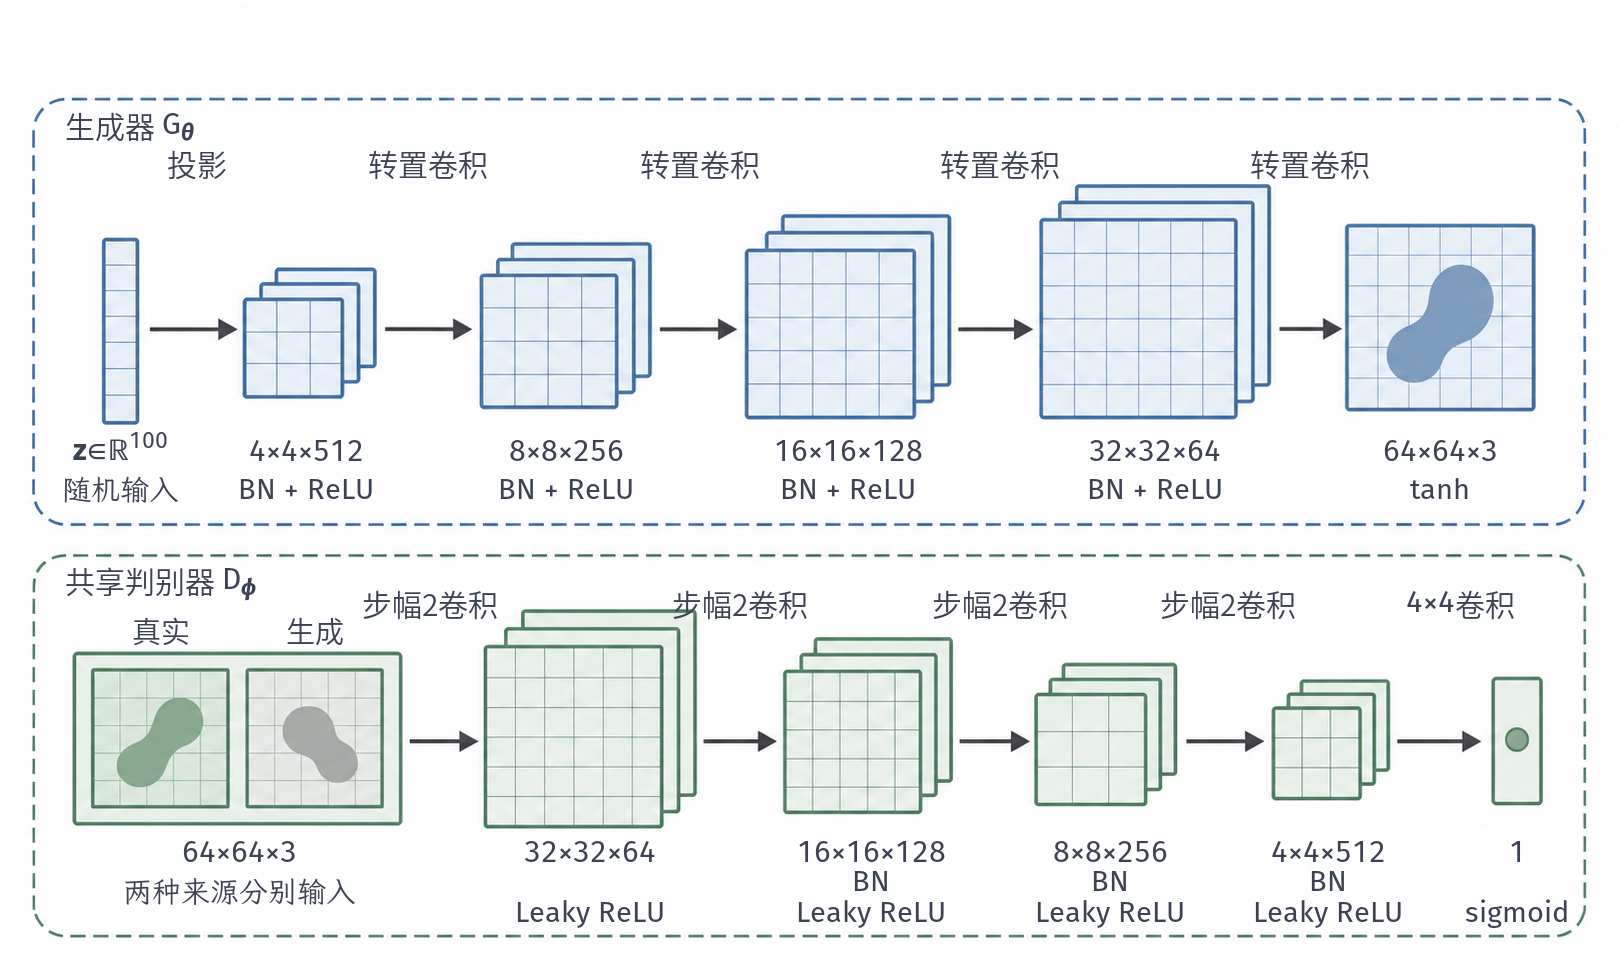
\includegraphics[width=150mm]{figures/08-neural-network-models/00-shared/generated/neural-generative-dcgan-architecture/figure.png}
  \caption{DCGAN的生成器逐级扩大空间尺寸，判别器通过带步幅卷积逐级缩小空间尺寸。通道数是一组教学配置，叠片只表示多通道。真实与生成图像是分别输入同一判别器的两种来源，不作通道拼接。隐藏层的归一化与激活标在尺寸链下方；生成器末层使用tanh，判别器末层以卷积得到单一得分，再经sigmoid输出来源概率。}
  \label{fig:neural-generative-dcgan-structure}
\end{figure*}

原DCGAN建议用带步幅卷积替代判别器的池化，用转置卷积完成生成器的尺寸扩展，并在多数层使用批量归一化。生成器隐藏层使用ReLU、末层使用tanh，判别器使用Leaky ReLU；生成器末层与判别器输入层不使用批量归一化。这些选择共同规定原论文的结构配置，其他尺寸和数据仍需重新设计通道数、层数及像素缩放。

批量归一化用于减小层间数值尺度变化给学习带来的困难。判别器的Leaky ReLU在负输入区间保留非零斜率，使这一段仍能回传梯度；生成器末层的tanh则把像素限制在$[-1,1]$，要求真实图像采用相容的像素范围。否则，判别器可能仅凭输出范围就区分两种来源。上述组合是原论文研究的架构选择，不能把其中一个组件单独当作训练稳定性的充分条件。DCGAN与普通GAN的关系，是给同一对抗学习方式配上适合图像的卷积表示，而不是提出了另一种生成任务\scite{neural-generative-radford2016}

\subsection{参数学习}
\label{sec:neural-generative-dcgan-learning}

DCGAN仍用真实与生成来源训练判别器，再沿判别器输入梯度训练生成器，目标沿用第\ref{sec:neural-generative-gan-learning}节。卷积核在空间位置间共享，其梯度从各使用位置汇总；生成器的上采样层同样通过反向传播学习如何组合局部特征。它改变候选图像的构造方式，没有另行引入一个与GAN不同的分布匹配目标。

生成时抽取随机输入，依次计算小特征图和上采样层，得到一张图像。若使用批量归一化，需要采用训练后确定的推理统计，避免同一随机输入的输出随生成批次组成而改变。插值两个随机向量可以观察生成器怎样连接输出，但一条平滑插值路径不能证明潜坐标已与语义因素一一对应。

\subsection{优化计算能力}
\label{sec:neural-generative-dcgan-computation-extension}

从低分辨率提高到高分辨率时，网络同时面对轮廓和细纹理，训练成本也迅速增加。渐进式增长GAN先在较低分辨率学习，再逐步接入更高分辨率的生成与判别层，使训练阶段逐步处理更细尺度；新旧分支在过渡阶段平滑混合，减少突然改变网络造成的扰动\scite{karras2018pggan}

渐进式增长调整的是训练过程中网络的规模与输出尺度。若最终结构固定，它不能自动说明最终候选空间比同样结构从头训练时更大；其主要作用在于组织高分辨率表示的学习过程。转置卷积还可能因贡献覆盖不均产生格状纹理，使用插值上采样后再卷积可以改变这种覆盖方式，但生成细节是否合理仍取决于训练目标与数据。

例如，先生成$8\times8$图像时，模型只能表示大致位置和颜色；接入$16\times16$层后，才有更多空间位置表示边缘。过渡时同时保留旧路径经上采样得到的图和新路径得到的图，再逐步提高新路径的权重；判别器的输入路径也作相应过渡。这样可以先保留已经形成的粗尺度组织，再学习新增细节。它针对的是高分辨率训练过程，和下一节通过改变比较准则获得不同梯度信号的思路可以结合。

图~\ref{fig:neural-generative-progressive-structure}进一步展开从$16\times16$到$32\times32$的过渡。生成器需要衔接的是两种像素输出，判别器需要衔接的是新旧图像入口；后者先把两条路径变成相同分辨率、相同通道数的特征，再送入原有的判别层。因此，两方的混合发生在不同的计算对象上，不能把判别器的过渡理解成两个最终评分的平均。
\begin{figure}[!htb]
  \centering
  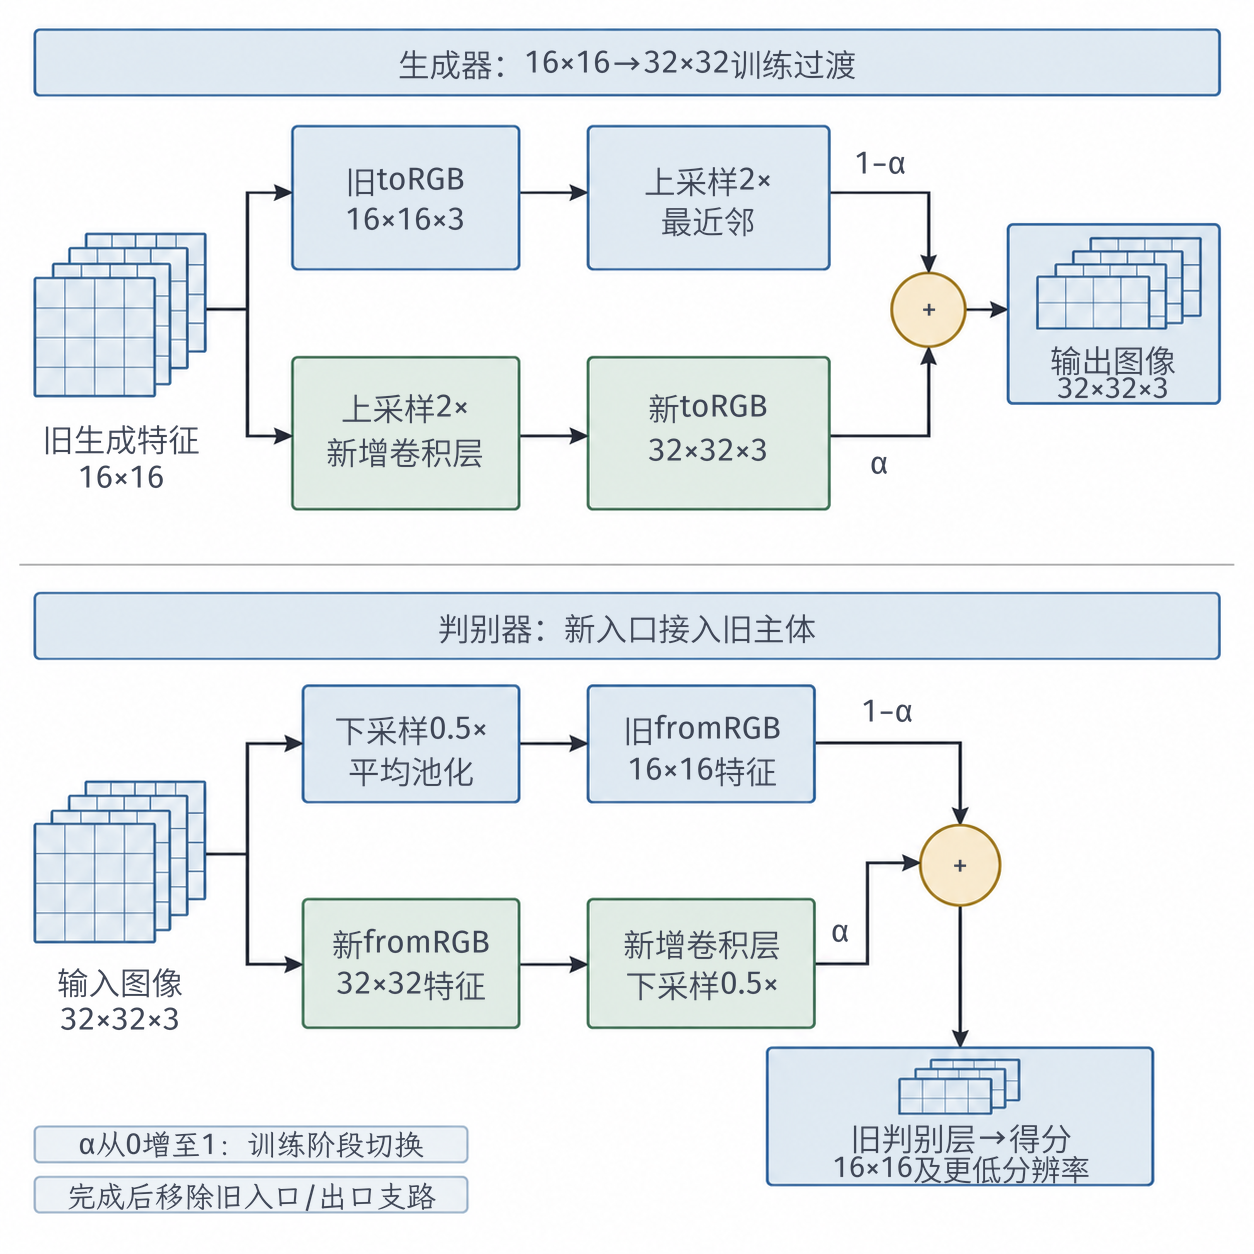
\includegraphics[width=112mm]{figures/08-neural-network-models/00-shared/generated/neural-generative-architectures/progressive/figure.png}
  \caption{渐进式增长GAN增添分辨率层时的局部结构。生成器混合上采样后的旧输出与新输出；判别器先把两种入口转换成相同分辨率的特征，再混合后送入旧主体。权重$\alpha$在训练过渡阶段从0增至1，完成后去掉旧入口和旧输出支路；旧主体仍继续训练，并非保留两个独立模型作集成。toRGB与fromRGB是图像通道与特征通道之间的$1\times1$卷积映射。}
  \label{fig:neural-generative-progressive-structure}
\end{figure}
\FloatBarrier
\section{Wasserstein生成对抗网络}
\label{sec:neural-generative-wgan}

\subsection{网络结构与比较目标}
\label{sec:neural-generative-wgan-structure}

GAN思想虽好，实践中却常出现训练难以推进的问题，根源藏在它用来衡量两分布差距的那个量（JS散度）上。考虑一个极端但说明问题的情形：真实分布和生成分布的支撑几乎不重叠——在高维图像空间里这才是常态，两团点云极难真正相交。此时判别器几乎能做到100\%正确分类，而“能否完美分类”这件事对两团分布相距多远毫不敏感。例如，真实数据恒为0，生成数据恒为$a\ne0$；两种来源可以完全区分，而把$a$从1改为0.01已经明显减小生成偏差。原始GAN在理想判别器下的比较值对所有$a\ne0$都相同，不能反映这段移动的距离。生成器收到的信号因此常常要么太强（完美分类、目标饱）、要么突然消失，无法得到“你离目标还有多远”的平滑指引。下面先用数学看清这个理想值为什么不随距离变化，再引出改用“搬运距离”的WGAN。

要看清这个理想值为什么不随距离变化，可以先固定生成器及其分布$Q$，只求判别器能够达到怎样的来源比较值。这里暂不限制判别器的网络结构，而允许任意可测的来源概率函数$D$。这样得到的理想上界，随后才能与有限网络实际学到的评分区分。

真实观测可能连续，也可能像上面的例子一样集中在几个点上。为了在同一种写法下比较二者，取参照测度$\mu=P+Q$，并记相对于它的密度为$p=\mathrm{d}P/\mathrm{d}\mu$和$q=\mathrm{d}Q/\mathrm{d}\mu$。二者都用同一份参照质量计量，因此$p+q=1$在$\mu$几乎处处成立；$\mu$的总质量为2。这样的密度也能表示点分布，无须假定存在相对于通常体积的连续密度。把式~\eqref{eq:neural-generative-gan-game}的总体目标按这份参照改写，暂记为
\begin{equation}
  \label{eq:neural-generative-gan-density-objective}
  V(Q,D)=\int\bigl[p(\bm{x})\log D(\bm{x})
      +q(\bm{x})\log\{1-D(\bm{x})\}\bigr]\,\mathrm{d}\mu(\bm{x}).
\end{equation}
固定$Q$后，$p,q$已经确定；不受网络结构限制的$D$可以在各位置选择来源概率。对某个位置，暂将$p(\bm{x}),q(\bm{x})$简写为$p,q$，把待选概率写为$r\in(0,1)$。该位置的目标是$h(r)=p\log r+q\log(1-r)$，其导数为
\[
  h'(r)=\frac{p}{r}-\frac{q}{1-r},\qquad
  h''(r)=-\frac{p}{r^2}-\frac{q}{(1-r)^2}.
\]
当$p,q$都为正时，二阶导数为负，解$h'(r)=0$得到唯一最优概率。将这一选择写回原位置，得到
\begin{equation}
  \label{eq:neural-generative-gan-optimal-discriminator}
  D^*(\bm{x})=\frac{p(\bm{x})}{p(\bm{x})+q(\bm{x})}.
\end{equation}
它表示该位置的总来源质量中，真实来源占多少。若只有真实来源有质量，最优选择趋向1；若只有生成来源有质量，最优选择趋向0。前面将$D$的输出规定在开区间$(0,1)$，所以这两种端点作为极限理解，理想目标使用上确界。两密度共同为零的位置不影响积分，判别值可任意指定。

逐点最优给出了整体目标的上界，还需要确认允许的判别函数能够逼近它。对$0<\varepsilon<1/2$，取$D_{\varepsilon}=\varepsilon+(1-2\varepsilon)D^*$，其输出始终在$(0,1)$内。它满足$D_{\varepsilon}\geq(1-2\varepsilon)D^*$以及$1-D_{\varepsilon}\geq(1-2\varepsilon)(1-D^*)$；分别取对数，再对真实项和生成项积分，就有
\[
  0\leq V(Q,D^*)-V(Q,D_{\varepsilon})
       \leq-2\log(1-2\varepsilon)\longrightarrow0.
\]
这里$V(Q,D^*)$表示允许极限端点的理想积分，零质量项按极限理解。右端的系数2来自两种来源各有总质量1。因而即使端点不能取到，仍能用允许的$D_{\varepsilon}$任意逼近这个值，逐点最优的积分确实给出总体目标的上确界。

令$S=(P+Q)/2$为两分布的等权混合，其相对于$\mu$的密度为$s=(p+q)/2$。把$D^*$代回目标时，真实项中的$\log\{p/(p+q)\}$可以写成$\log(p/s)-\log2$，生成项同理。$P,Q$的质量各为1，所以两个常数项合计为$-\log4$；密度为零的项按$0\log0=0$的极限约定处理。于是
\begin{equation}
  \label{eq:neural-generative-gan-js-value}
  \begin{aligned}
  \sup_D V(Q,D)
    ={}&\int p\log\frac{p}{p+q}\,\mathrm{d}\mu
       +\int q\log\frac{q}{p+q}\,\mathrm{d}\mu\\
    ={}&-\log4+\operatorname{KL}(P\|S)
       +\operatorname{KL}(Q\|S).
  \end{aligned}
\end{equation}
这两份KL之和把理想来源比较接到了Jensen--Shannon散度（Jensen--Shannon divergence, JS）。JS用两分布各自相对于混合分布的KL散度取平均：$\operatorname{JS}(P,Q)=\tfrac12\operatorname{KL}(P\|S)+\tfrac12\operatorname{KL}(Q\|S)$。若不限制判别函数的表达形式，原GAN判别目标对所有可测判别函数的上确界因而为$-\log4+2\operatorname{JS}(P,Q)$。这里计算的是固定生成分布后的最佳判别值，有限网络和有限次判别器更新还未必能达到它\scite{pgm-generative-goodfellow2014}

两分布相同时JS为0，式~\eqref{eq:neural-generative-gan-optimal-discriminator}在有质量的位置给出$D^*=1/2$。这也解释了前面所说的理想分布匹配点：两来源在同一位置提供相同的质量。支撑完全不相交时，在各自有质量的位置，混合密度都是本来源密度的一半，所以两份KL均为$\log2$，JS也为$\log2$。因此，前面的两个点只要尚未重合，这个理想值就不能区分它们相距1还是0.01；有限网络和非饱和更新的实际梯度则还取决于具体参数，不能直接从这个例子断言所有GAN训练都会停滞。

为了得到一个对“相距多远”连续敏感的量，可以换一个非常物理的视角：把生成分布想象成一堆土，真实分布是目标形状的坑，衡量差距就是计算平均最少要把每捧土搬多远才能填成目标形状。这就是Wasserstein距离（也叫推土机距离，earth-mover distance），它的巨大优点是：即使两团土完全不重叠，搬动距离依然随位置连续变化，$a$离0越近差距越小，从而给生成器提供平滑的学习信号。Arjovsky、Chintala和Bottou在2017年提出\term{Wasserstein生成对抗网络}（Wasserstein generative adversarial network, WGAN），用把生成分布搬到真实分布所需的平均距离提供目标。假设$P$和$Q$在欧氏空间上且一阶矩有限，记$\Pi(P,Q)$为边缘分别为$P,Q$的联合分布集合，则
\begin{equation}
  \label{eq:neural-generative-wasserstein}
  W_1(P,Q)=\inf_{\pi\in\Pi(P,Q)}
    \mathbb{E}_{(\bm{X},\bm{Y})\sim\pi}
       \lVert\bm{X}-\bm{Y}\rVert_2.
\end{equation}
联合分布规定哪些质量从什么位置移到什么位置，下确界选取平均移动距离最小的安排。记$\delta_a$为概率全部集中在$a$的点分布。对前面的两个点分布，唯一的搬运就是把$a$移到0，故$W_1(\delta_0,\delta_a)=|a|$。图~\ref{fig:neural-generative-distance}比较两种准则在这个例子上的变化\scite{neural-generative-arjovsky2017}
\begin{figure}[htbp]
  \centering
  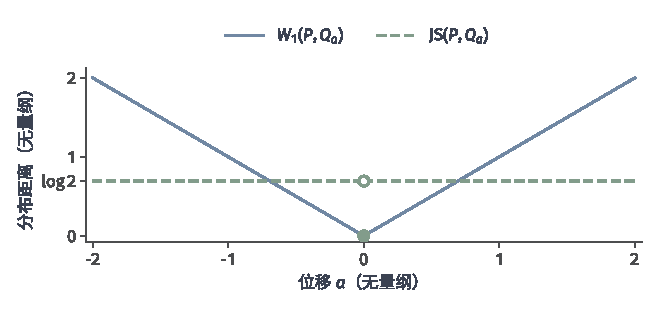
\includegraphics[width=112mm]{figures/08-neural-network-models/00-shared/matplotlib/neural-generative-objectives/distance/figure.pdf}
  \caption{真实分布$\delta_0$与生成分布$\delta_a$的比较。$a\ne0$时两分布支撑不相交，Jensen--Shannon散度恒为$\log2$；$a=0$时为0。Wasserstein距离为$|a|$，随生成位置连续变化。断开的点与线用于表示JS在0处的不连续，所有量均由解析式计算。}
  \label{fig:neural-generative-distance}
\end{figure}

搬运距离的原始定义需要枚举所有可能的“搬运方案”再取最小值，这对高维图像根本无法直接优化。所幸它有一个对偶形式，可以把“找最优搬运”转化为“找一个评分函数”，这才让神经网络有了用武之地：WGAN利用$W_1$的对偶形式，把比较转成函数评分。不过这个评分函数不能任意陡——若不加限制，它可以在真实样本和生成样本之间给出任意大的分差，差距就失去意义，所以必须要求评分随输入平滑变化（满足1-Lipschitz）：
\begin{equation}
  \label{eq:neural-generative-wgan-dual}
  W_1(P,Q)=\sup_{\operatorname{Lip}(f)\leq1}
    \{\mathbb{E}_{P}f(\bm{X})-\mathbb{E}_{Q}f(\bm{X})\}.
\end{equation}
允许函数满足$|f(\bm{x})-f(\bm{y})|\leq\lVert\bm{x}-\bm{y}\rVert_2$，即输入移动一段距离时，评分不能变化得更快。这个约束避免把任意微小来源差异放大成无限大的评分差。

这种评分限制为什么会与搬运距离联系起来？任取一个允许的$f$和一个边缘为$P,Q$的联合分布$\pi$。因为联合分布保留了两边的边缘，分别计算两组评分均值，与在配对后计算评分差的均值相同；逐对使用上述变化幅度限制，就得到
\[
  \begin{aligned}
  \mathbb{E}_P f(\bm{X})-\mathbb{E}_Q f(\bm{Y})
    &=\mathbb{E}_{\pi}\{f(\bm{X})-f(\bm{Y})\}\\
    &\leq\mathbb{E}_{\pi}\lVert\bm{X}-\bm{Y}\rVert_2.
  \end{aligned}
\]
有限一阶矩使这些1-Lipschitz评分的期望存在。这个不等式对每一种搬运安排都成立，所以评分差至多为最小平均搬运距离。式~\eqref{eq:neural-generative-wgan-dual}进一步说明，在全部允许评分中取上确界，可以达到这个距离；反向等号由Wasserstein距离的对偶定理给出，单靠上面的不等式还不能推出。

仍以$P=\delta_0,Q=\delta_a$为例。$a\ne0$时，具体取$f(t)=-\operatorname{sign}(a)t$，其中$\operatorname{sign}(a)$在$a>0$时为1、在$a<0$时为$-1$。这个函数的斜率绝对值为1，属于允许集合，而且$f(0)-f(a)=|a|$；$a=0$时取常数函数即可得到零评分差。一个允许的评分函数由此可以让从$a$移动到0时的评分差达到$|a|$，却不能为了把两种来源分开而在两点间无限增大斜率。改变$a$的位置就会改变最大的评分差。WGAN由此把“这两个来源能否完全分类”换成“在受限变化的评分下，两组观测还差多少”，让不同距离的生成偏差有机会形成不同的学习信号。

WGAN用实值网络$f_{\bm{\phi}}:\mathbb{R}^{d}\to\mathbb{R}$近似上述评分函数，称为\term{评价器}（critic）。评价器定义在包含观测空间的环境空间上，可以计算图像输入及后面插值点的评分。它没有把输出限制在$[0,1]$，也不估计来源概率。对实际网络集合$\mathcal{F}$，训练比较的是
\begin{equation}
  \label{eq:neural-generative-wgan-objective}
  \min_{\bm{\theta}}\max_{f_{\bm{\phi}}\in\mathcal{F}}
  \left\{\mathbb{E}_{P}f_{\bm{\phi}}(\bm{X})
  -\mathbb{E}_{\nu}f_{\bm{\phi}}(G_{\bm{\theta}}(\bm{Z}))\right\}.
\end{equation}
若允许全部1-Lipschitz函数并求得内层上确界，就得到$W_1$。实际网络族能否达到这个值，还取决于它是否包含相应的最优评分函数，以及内层求解是否充分。有限网络给出受其辨别能力限制的比较，不能把每次训练中的评分差直接称为精确Wasserstein距离。

图~\ref{fig:neural-generative-wgan-structure}显示这个改动在网络中的位置。生成器仍可以采用DCGAN的卷积与上采样路径，改变的是判别一方的末层和学习目标：去掉来源sigmoid，直接输出实数评分，并在训练中限制评分随输入变化的幅度。图像层级与分布比较因此是两个可以分别选择的设计方向，WGAN不要求把卷积生成器换成某一种新的固定骨架。
\begin{figure*}[htbp]
  \centering
  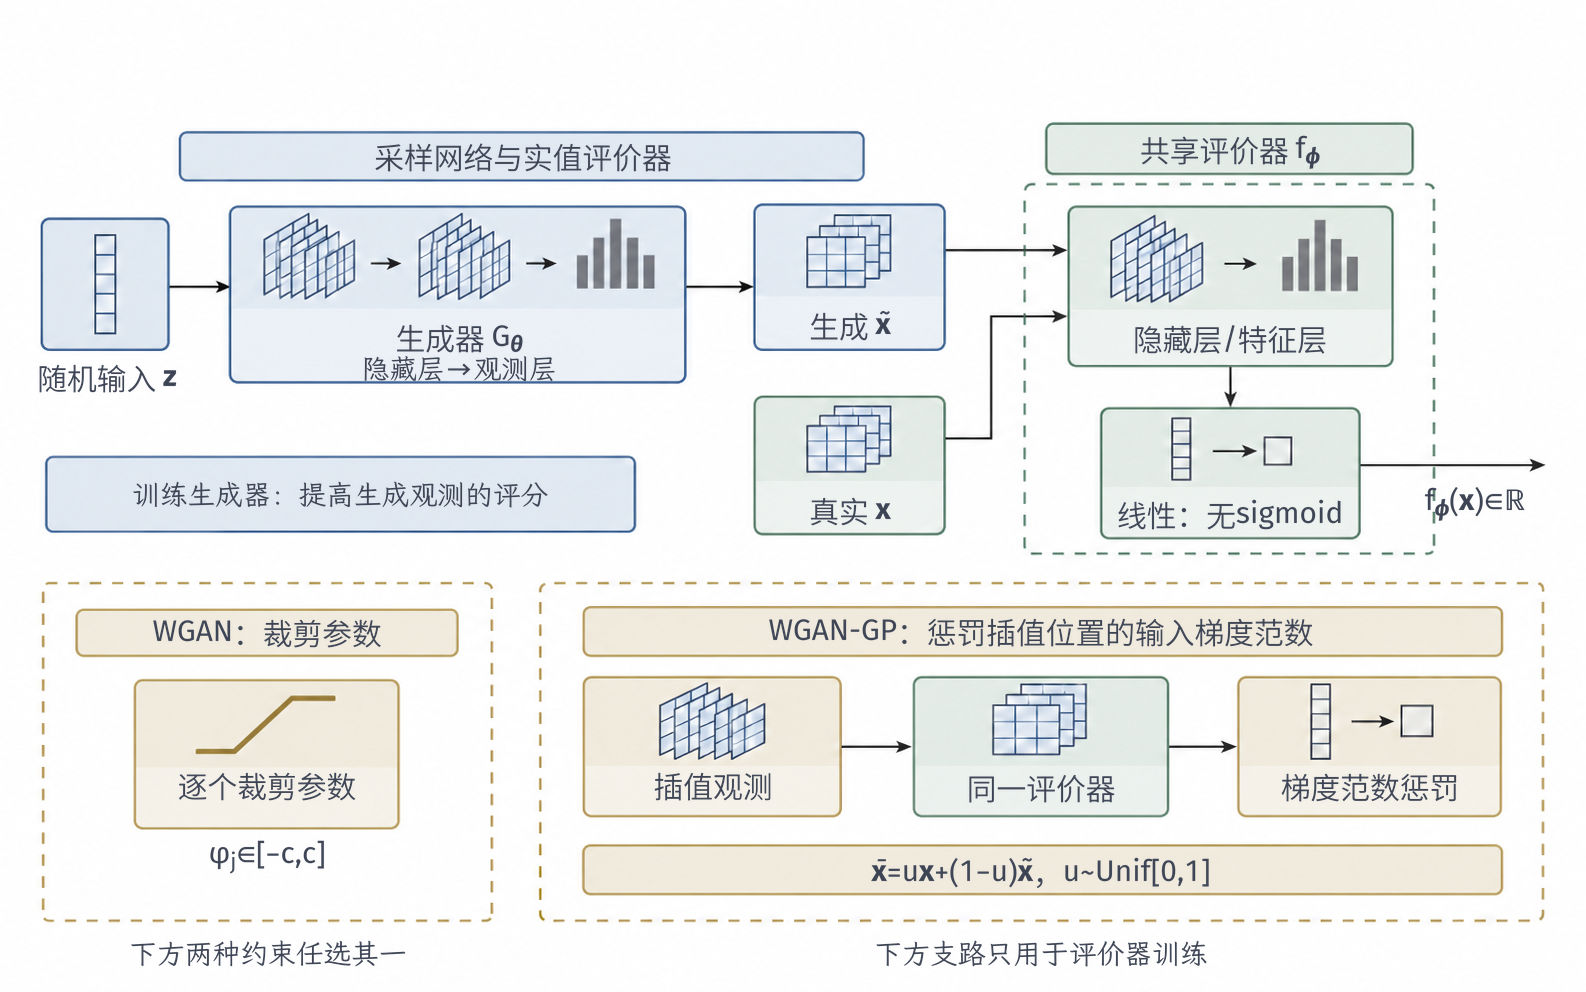
\includegraphics[width=150mm]{figures/08-neural-network-models/00-shared/generated/neural-generative-architectures/wgan/figure.png}
  \caption{WGAN将来源概率改为不经过sigmoid的实数评分。下方是两种评价器训练约束：原WGAN裁剪评价器参数；WGAN-GP在真实与生成观测之间抽取插值点，再惩罚同一评价器在这些点上的输入梯度范数偏离1。下方支路只用于评价器训练，未增加生成器层，也不是生成样本的输出后处理。}
  \label{fig:neural-generative-wgan-structure}
\end{figure*}

\subsection{参数学习}
\label{sec:neural-generative-wgan-learning}

评价器希望真实样本评分高、生成样本评分低，因此最小化$\mathbb{E}_{\nu}f(G(\bm{Z}))-\mathbb{E}_{P}f(\bm{X})$；生成器则希望生成评分提高，最小化$-\mathbb{E}_{\nu}f(G(\bm{Z}))$。两方仍交替更新，评价器通常先更新若干次，再给生成器一次更新。生成器的梯度来自实值评分对图像的导数，不再经过来源sigmoid。

如果生成器刚改变了输出，评价器之前学到的评分未必仍能代表当前两组样本的差异。给评价器多次更新，是希望它先适应新的生成分布，再提供生成器的更新方向；更新预算仍是需要选择的训练设置。增加评价器步数会增加每轮成本，也不能代替对其表示能力和约束实现的检查。生成时照旧只计算$G(\bm{z})$，不需要搬运训练样本，也不需要搜索某个最大评分的图像。

理论要求评分函数满足1-Lipschitz，但怎么在一个普通神经网络上强制这个约束，本身是个工程难题。原始WGAN采用最简单粗暴的办法：每次更新后，把评价器的每个参数都裁剪（clip）到一个固定的小区间$[-c,c]$内。原始WGAN把评价器参数逐元素裁剪到一个有限区间，以限制评分变化。参数有界确实会限制一组给定网络的Lipschitz常数，却一般不使该常数恰好为1；裁剪区间过小还会压缩可用评分函数，使评价器难以表达所需差异。它是可执行的近似约束，不等于直接求解式~\eqref{eq:neural-generative-wgan-dual}的全部函数。

权重裁剪没有直接考察网络对图像究竟有多敏感。以$\ell$层标量线性网络为例，若每个权重的绝对值都不超过$c_0<1$，评分对输入的导数绝对值就不超过$c_0^\ell$；层数增加时，这条路径给生成器的梯度可能很弱。真实网络还包含多通道与非线性运算，但这个简单计算已能说明：限制每个参数与保留有用的输入梯度是不同要求。WGAN-GP承接这个约束实现问题，保留WGAN的实值评分和生成器更新，再改变如何限制评价器。

\subsection{优化计算能力}
\label{sec:neural-generative-wgan-computation-extension}

为了减少权重裁剪对评价器形状的限制，Gulrajani等在2017年提出带梯度惩罚的WGAN（WGAN with gradient penalty, WGAN-GP）。它在真实样本与生成样本之间抽取插值点，直接惩罚评价器在这些点上的梯度长度偏离1\scite{neural-generative-gulrajani2017}

为什么把梯度长度的目标设为1？回到真实位置为0、生成位置为$a>0$的例子，评分函数$f(t)=-t$能给出恰好为$a$的评分差，在两点之间的梯度长度也是1。若这段评分几乎不变，它就不能反映两个位置相隔多远。WGAN-GP希望限制过大的评分变化，同时保留能区分偏差的梯度，因此也惩罚过小的梯度；这是对插值位置施加的训练要求，并不是说所有允许的评分函数在所有位置都应有单位梯度。

独立抽取$\bm{X}\sim P$、$\bm{Z}\sim\nu$与$U\sim\operatorname{Unif}[0,1]$，令$\overline{\bm{X}}=U\bm{X}+(1-U)G_{\bm{\theta}}(\bm{Z})$。这些点在环境空间$\mathbb{R}^{d}$中构造，不必是真实图像，也不必位于真实或生成数据的支撑中。评价器最小化
\begin{equation}
  \label{eq:neural-generative-wgan-gp}
  \begin{aligned}
  L_f={}&\mathbb{E}_{\nu}f_{\bm{\phi}}(G_{\bm{\theta}}(\bm{Z}))
        -\mathbb{E}_{P}f_{\bm{\phi}}(\bm{X})\\
        &+\lambda\mathbb{E}
        \bigl(\lVert\nabla_{\bm{x}}
                    f_{\bm{\phi}}(\overline{\bm{X}})\rVert_2-1\bigr)^2,
        \qquad\lambda>0.
  \end{aligned}
\end{equation}
固定生成器后，对这个目标的样本近似反向传播，更新评价器；生成器仍最小化负评分。计算惩罚需要对输入求导，再把惩罚回传到评价器参数，因而增加训练计算量。

插值点属于训练约束的采样路径，不是生成器产生图像时必须经过的一层。若真实样本为$\bm{x}$、生成样本为$\widetilde{\bm{x}}$，抽到$U=1/2$时就在两者的中点检查评价器变化；换一组端点或插值系数，就检查另一处。更新评价器时固定生成图及插值点，再计算相对于图像输入的梯度长度。为使这项惩罚针对单个输入，原WGAN-GP评价器不使用把同批样本相互耦合的批量归一化；这与DCGAN的原始判别器配置有实质差别\scite{neural-generative-gulrajani2017}

梯度惩罚把近似约束放在抽取的插值位置，允许权重保留更多变化，原论文在所测试的网络与数据上改善了训练稳定性。惩罚趋向梯度长度为1，而全局1-Lipschitz条件要求长度不超过1；有限插值点也没有覆盖全部输入。WGAN-GP因此不能提供全局约束已经严格满足、模式坍缩已经消失或交替训练必然收敛的保证。

\section{条件生成与图像转换}
\label{sec:neural-generative-conditional}

从随机输入生成一张合理的图像，还没有回答它是否满足当前要求。我们可能要指定数字类别，也可能要把一张分割图转换成照片；后一种任务还要求建筑、道路与天空的位置随输入保留。条件提供了应当生成什么的信息，而训练数据是否给出输入与目标的对应关系，又决定了可以怎样约束转换。

\subsection{条件生成对抗网络}
\label{sec:neural-generative-cgan}

无条件GAN混合学习各类数字的写法。若现在只需要数字“3”，我们可以不断生成并筛选，但大量输出会被丢弃，已有的类别标签也没有参与学习。希望指定类别后直接生成，同时保留这一类中粗细、倾斜和笔画形状的变化，就需要把“生成哪一类”和“生成这一类的哪一种写法”分开交给两个输入。

Mirza和Osindero在2014年提出\term{条件生成对抗网络}（conditional generative adversarial network, cGAN），把已知条件同时加入生成器与判别器。令$C$为类别、属性或其他已知输入，真实训练观测为$(\bm{X},C)\sim P_{\bm{X},C}$；$P_C$表示条件变量本身在总体中的分布。生成器接收随机输入$\bm{Z}\sim\nu$和条件$C$，输出$G_{\bm{\theta}}(\bm{Z},C)$。判别器接收图像与条件组成的观测，判断它们是否共同来自真实数据\scite{neural-generative-mirza2014}

cGAN的来源比较需要两方都能看到条件。假设训练集中的“3”和“8”各占一半，生成器却在收到“3”时输出“8”、收到“8”时输出“3”。只看图像的判别器仍会看到一半“3”、一半“8”，无法通过这次比较发现类别被交换。接收图像与标签的判别器则可以检查“这张图是否像标签所指的数字”。图~\ref{fig:neural-generative-cgan-structure}可以用来对照条件进入两网络的位置；同一个条件既规定生成要求，也参与判断这个要求是否满足。
\begin{figure*}[tbp]
  \centering
  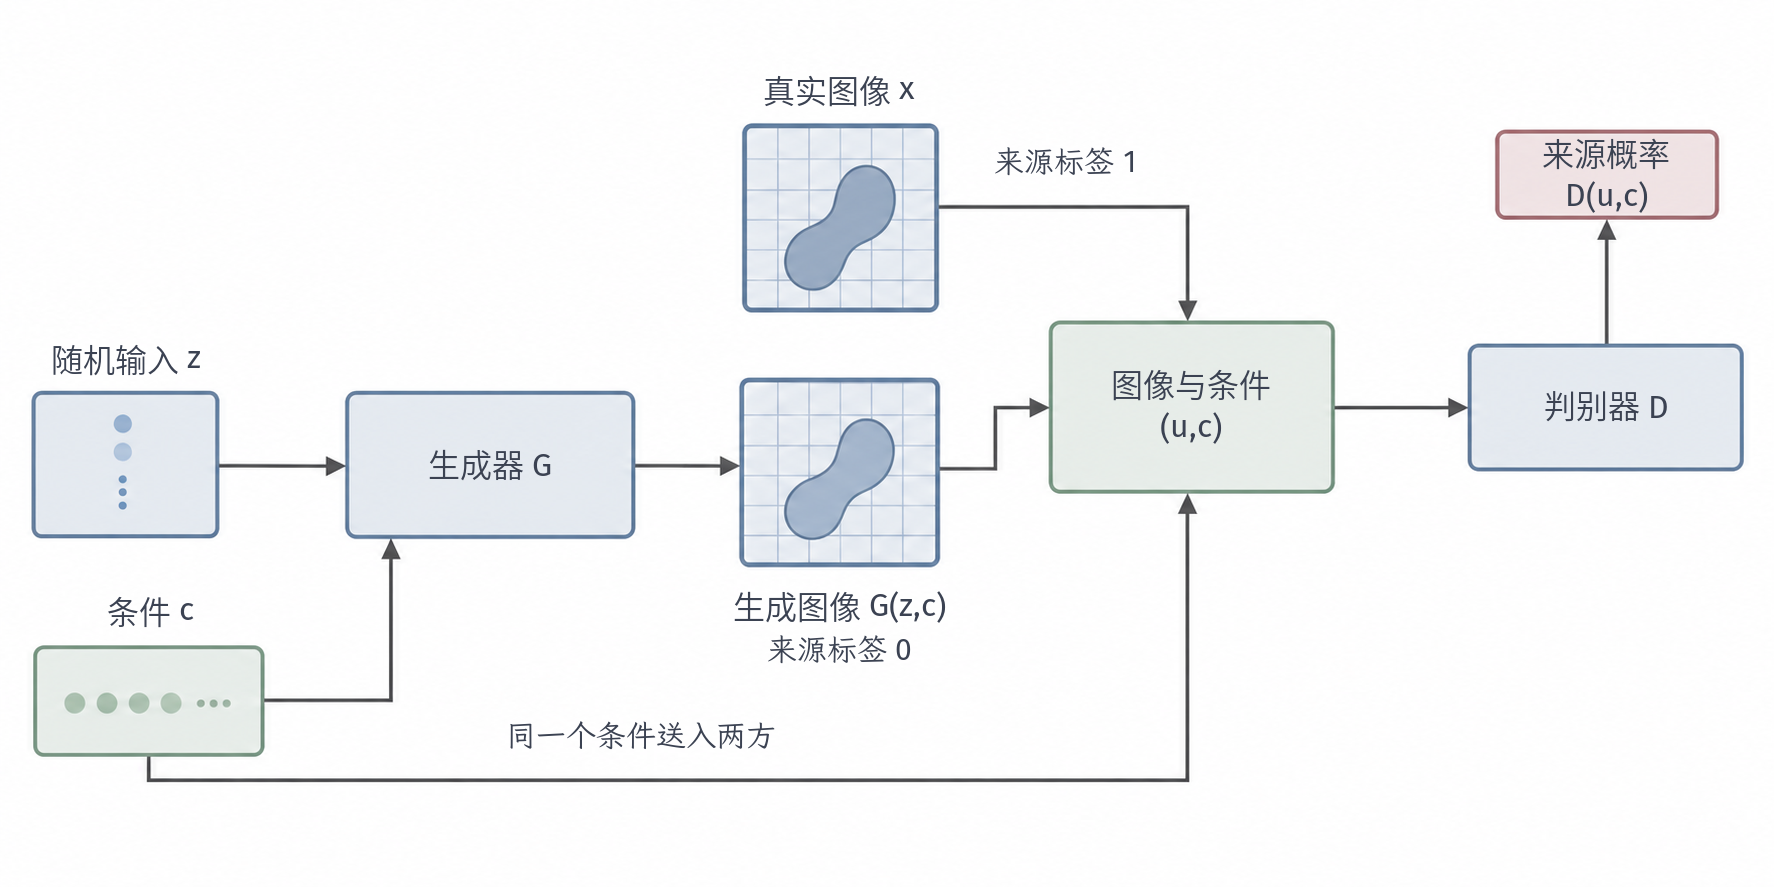
\includegraphics[width=156mm]{figures/08-neural-network-models/00-shared/generated/neural-generative-architectures/cgan/figure.png}
  \caption{条件GAN的两方输入。$G$和$D$的内部可沿用前述GAN骨架，这里突出新增的条件接入。条件$c$同时送入生成器和判别器；判别器检查的是图像与条件是否共同来自真实数据。图中$\bm u$取真实图像$\bm x$或生成图像$G(\bm z,c)$，对应来源标签分别为1与0，两条图像支路表示两类训练样本。结构依据Mirza和Osindero（2014）。}
  \label{fig:neural-generative-cgan-structure}
\end{figure*}

对真实图像与条件计算来源判别项，对生成图像与同一条件计算另一项，就得到
\begin{equation}
  \label{eq:neural-generative-cgan-objective}
  \begin{aligned}
  \min_{\bm{\theta}}\max_{\bm{\phi}}\quad
  &\mathbb{E}_{(\bm{X},C)\sim P_{\bm{X},C}}
      \log D_{\bm{\phi}}(\bm{X},C)\\
  &+\mathbb{E}_{C\sim P_C,\bm{Z}\sim\nu}
      \log\{1-D_{\bm{\phi}}(G_{\bm{\theta}}(\bm{Z},C),C)\}.
  \end{aligned}
\end{equation}
这里的$\bm{Z}$与$C$独立抽取。真实与生成观测使用相同的条件变量分布$P_C$，使判别器比较的是图像与条件的联合关系，而不能仅凭两批数据的类别比例区分来源。在理想联合分布匹配时，每个具有正概率的离散类别也匹配其类内分布；对连续条件，这一说法限于$P_C$几乎处处的条件。

训练时从样本对$(\bm{x}_i,c_i)$取一个小批量，再为这些条件抽取随机输入。固定生成器，判别器学习区分$(\bm{x}_i,c_i)$与$(G_{\bm{\theta}}(\bm{z}_i,c_i),c_i)$；固定判别器，生成器沿图像输入的梯度调整输出。可以沿用第\ref{sec:neural-generative-gan-learning}节的非饱和生成损失。类别通常先转成独热向量或嵌入，再与网络特征结合；条件的表示和接入位置可以改变，但两方需要获得同一条件的信息。

生成时指定$c$，反复抽取$\bm{z}$并计算$G_{\bm{\theta}}(\bm{z},c)$，判别器不再参与输出。cGAN把无条件采样扩展为有条件采样，仍保留GAN的来源比较与交替学习。它没有规定类内每一种写法都必须出现，稀少条件也只有较少训练样本；标签控制与类内覆盖因此仍需分别检查。

\subsection{有配对样本的图像转换}
\label{sec:neural-generative-pix2pix}

把语义分割图变成照片时，条件本身是一张图像。假设输入规定了道路和建筑的边界，目标是同一场景的照片，生成器既要保留这些位置，又要补出墙面、树叶和路面的纹理。逐像素重建可以利用位置对应，但每个位置的偏差并不足以描述“这些像素合起来是否像一块真实墙面”。仅检查照片是否合理，又可能允许生成器改变输入规定的内容。

Isola、Zhu、Zhou和Efros于2016年公开、2017年发表的pix2pix，将图像作为cGAN的条件，并把条件对抗学习与配对重建放在同一个目标中。令随机图像对$(\bm{A},\bm{B})$表示输入图与对应目标图，生成器从$\bm{A}$构造目标图，判别器比较真实图像对$(\bm{A},\bm{B})$与生成图像对$(\bm{A},G(\bm{A}))$。这样，判别器学到的来源判断也取决于输入，不能只检查输出图的外观\scite{neural-generative-isola2017}

为了把输入的位置关系传到输出，生成器采用带跨层连接的U-Net。编码器逐步缩小空间尺寸，提取较大范围的关系，解码器再逐步恢复分辨率。若全部信息都必须经过最小尺寸的中间表示，细小边缘和位置需要被压缩后重新恢复；U-Net把编码器的特征直接接到相同分辨率的解码层，与该层特征沿通道拼接。解码层因而可以同时使用较大范围的信息和仍有明确位置的细节，而不必仅凭压缩表示重建每条边缘。

保留输入信息还不能决定怎样评价生成纹理。pix2pix采用\term{局部块判别器}（PatchGAN），在多个重叠感受野内检查输入与输出的图像块，训练时汇总各位置的来源判别损失。原论文的一种配置使用$70\times70$的感受野。对于墙面这样的区域，局部块可以检查边缘、颜色变化和纹理是否共同呈现真实照片的结构；它不必为每种纹理手工规定像素误差。图~\ref{fig:neural-generative-pix2pix-structure}可沿输入信息的跨层传递和局部判别两条路径阅读：前者提供可用的位置细节，后者对生成的局部组合提出要求。
\begin{figure*}[tbp]
  \centering
  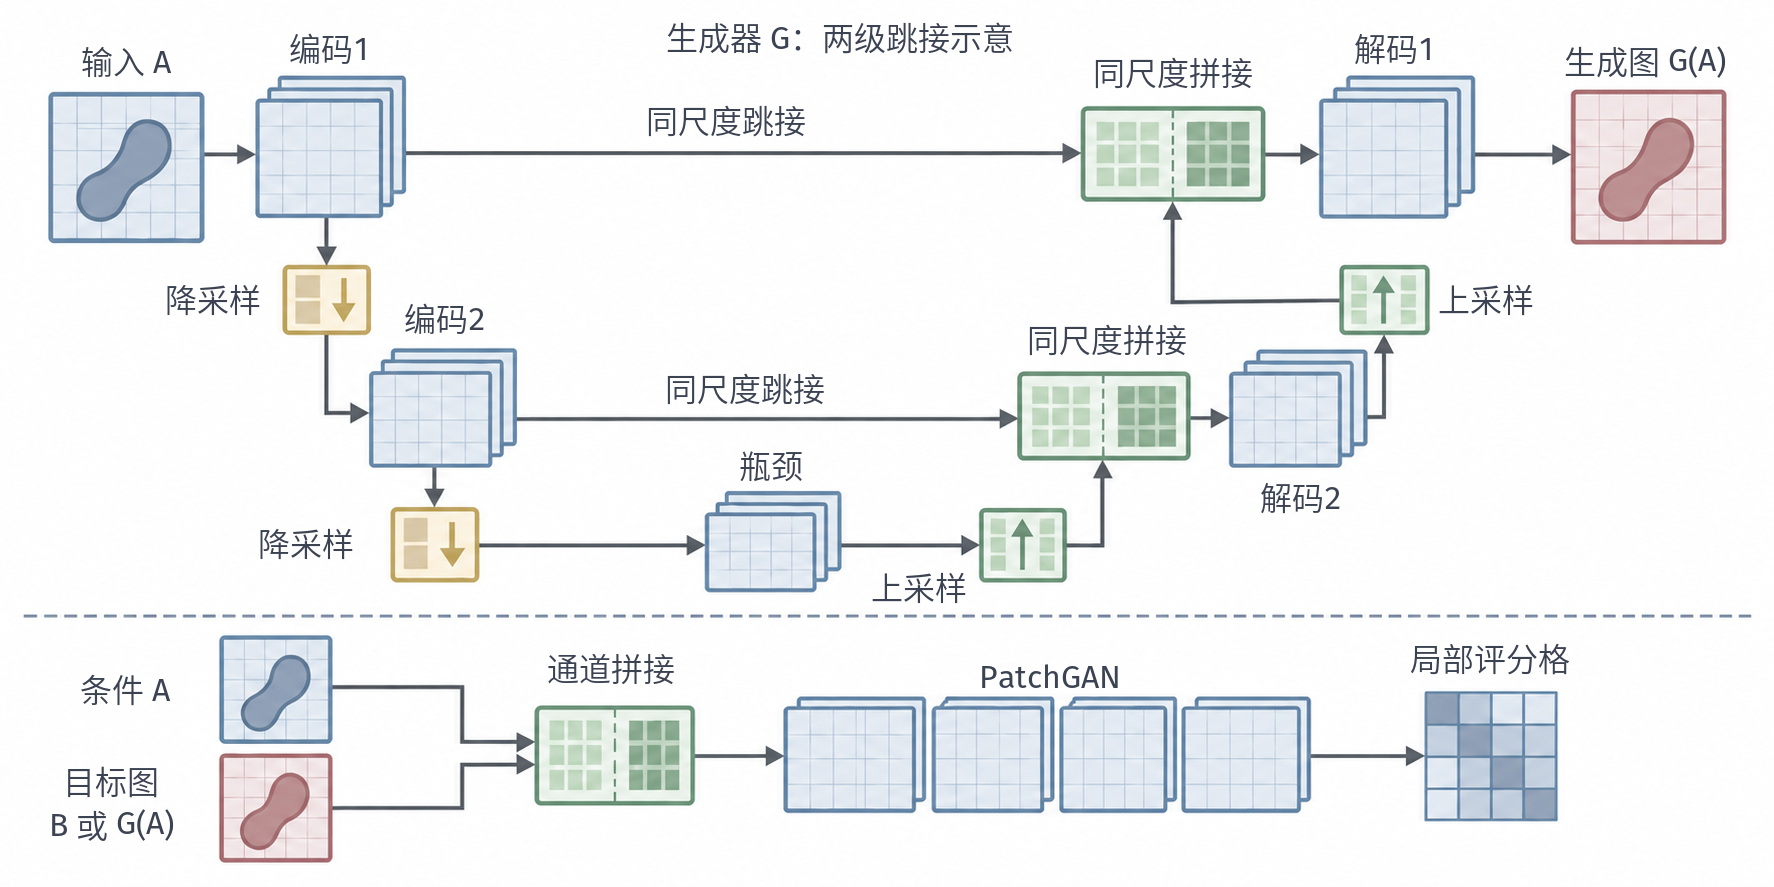
\includegraphics[width=156mm]{figures/08-neural-network-models/00-shared/generated/neural-generative-architectures/pix2pix/figure.png}
  \caption{pix2pix的生成与条件判别。上方仅展开U-Net的两级跳接：编码特征与同尺度上采样结果先按通道拼接，再由解码层处理；下方把条件图$A$与真实目标$B$或生成结果$G(A)$共同送入PatchGAN，得到局部图像块的评分。网格、层数和特征片数量为机制示意，不表示原模型的实际尺寸；省略归一化、激活、Dropout及配对重建损失。结构依据Isola等（2017）。}
  \label{fig:neural-generative-pix2pix-structure}
\end{figure*}

配对目标图还提供了另一条直接约束：在相同位置，把生成像素与目标像素比较。下面暂时省略参数与dropout随机性，将生成器写为$G(\bm{A})$，并用单个来源概率$D$展示对抗项；PatchGAN实现对各局部位置的判别项取平均。保留dropout时，两类损失还应对它的随机源取期望。目标为
\begin{equation}
  \label{eq:neural-generative-pix2pix}
  \begin{aligned}
  \min_G\max_D\quad
    &\mathbb{E}_{\bm{A},\bm{B}}\log D(\bm{A},\bm{B})\\
    &+\mathbb{E}_{\bm{A}}\log\{1-D(\bm{A},G(\bm{A}))\}\\
    &+\lambda\mathbb{E}_{\bm{A},\bm{B}}
        \lVert\bm{B}-G(\bm{A})\rVert_1,
       \qquad\lambda>0.
  \end{aligned}
\end{equation}
$\ell_1$项把全部对应像素的绝对偏差相加，直接联系当前输入的目标图；对抗项则比较输入条件下的图像结构。U-Net的连接使信息能够传递，两个损失决定传来的信息怎样用于输出，它们承担的是不同环节。

这两项存在取舍。相同的分割图可能对应不同的光照与云层，训练中给出的照片只是其中一个结果。逐像素误差单独决定输出时，可以选择一种代表性结果或细节不足的折中纹理，并没有要求合成真实的纹理组合；对抗项为这些组合提供额外判断。增大$\lambda$会更重视当前配对目标的像素对应，减小$\lambda$则相对加强对抗项，但可能放松内容对应。$\ell_1$重建也可能抑制那些合理却不同于当前配对照片的变化，因此加入对抗项不等于已经学到同一输入的全部可能输出。

训练时，判别器只根据真实对和生成对更新；生成器则同时接收对抗损失与配对误差的梯度，实际可用非饱和形式计算生成端对抗损失。生成时直接把输入图送入训练好的生成器。原论文在训练和生成时都保留部分层的dropout以提供随机性，发现额外随机向量容易被网络忽略，而dropout带来的输出变化也比较有限。pix2pix适合配对转换；若要从同一输入产生明显不同的多个结果，还需要额外机制\scite{neural-generative-isola2017}

局部判别还有空间范围的限制：一块道路纹理合理，并不能说明道路在整张图中连通。较远位置之间的关系仍依赖生成器、条件和训练约束。与一般cGAN相比，pix2pix利用了图像的空间对应，专门组织信息传递和损失；这也使它依赖成对且对齐的训练样本。

\subsection{无配对样本的图像转换}
\label{sec:neural-generative-cyclegan}

若训练集只有一组马的照片和一组斑马的照片，便没有同一动物两种外观的配对目标。任取一张斑马照片与马照片逐像素比较，会把另一只动物的姿态和背景也当成当前输入应有的结果。另一方面，只要求输出像斑马，不能决定哪张输出应该对应当前这匹马。无配对转换因此缺少的是样本之间的对应依据。

Zhu、Park、Isola和Efros在2017年提出CycleGAN，用双向转换与来回重建补充这个约束。令两个图像域为$\mathcal{A},\mathcal{B}\subseteq\mathbb{R}^{d}$，随机观测为$\bm{A}\sim P_{\mathcal{A}}$与$\bm{B}\sim P_{\mathcal{B}}$。模型学习$G:\mathcal{A}\to\mathcal{B}$和$F:\mathcal{B}\to\mathcal{A}$。对一张马照片$\bm{a}$，先得到$G(\bm{a})$，再用$F$转换回来；原输入本身就成为这次来回转换的重建目标，不需要一张与它配对的真实斑马照片\scite{neural-generative-zhu2017}

两个方向还各自需要目标域的来源判断。$D_{\bm{B}}$比较真实斑马图与$G(\bm{A})$，$D_{\bm{A}}$比较真实马图与$F(\bm{B})$，因为两域的真实外观不同。这里判别器不接收一对输入与目标图来核验对应：训练数据没有提供这样的真实图像对。它们只检查转换图是否符合目标域，保留输入信息的要求交给来回重建。

来回重建的作用可以从信息丢失看出来。若两张姿态不同的马照片都被$G$映成同一张斑马图，确定性的$F$只能把这张图还原成一个结果，无法同时恢复两个输入。要求$F(G(\bm{a}))$接近$\bm{a}$，就限制了这类多对一丢失信息的转换。反方向也要求$G(F(\bm{b}))$接近$\bm{b}$，使斑马域的真实样本同样接受重建约束。这个要求称为\term{循环一致性}（cycle consistency）：两网络的来回转换应尽量恢复起点。图~\ref{fig:neural-generative-cyclegan-structure}可以分别追踪两条循环，以及每个方向通往其目标域判别器的路径。
\begin{figure*}[tbp]
  \centering
  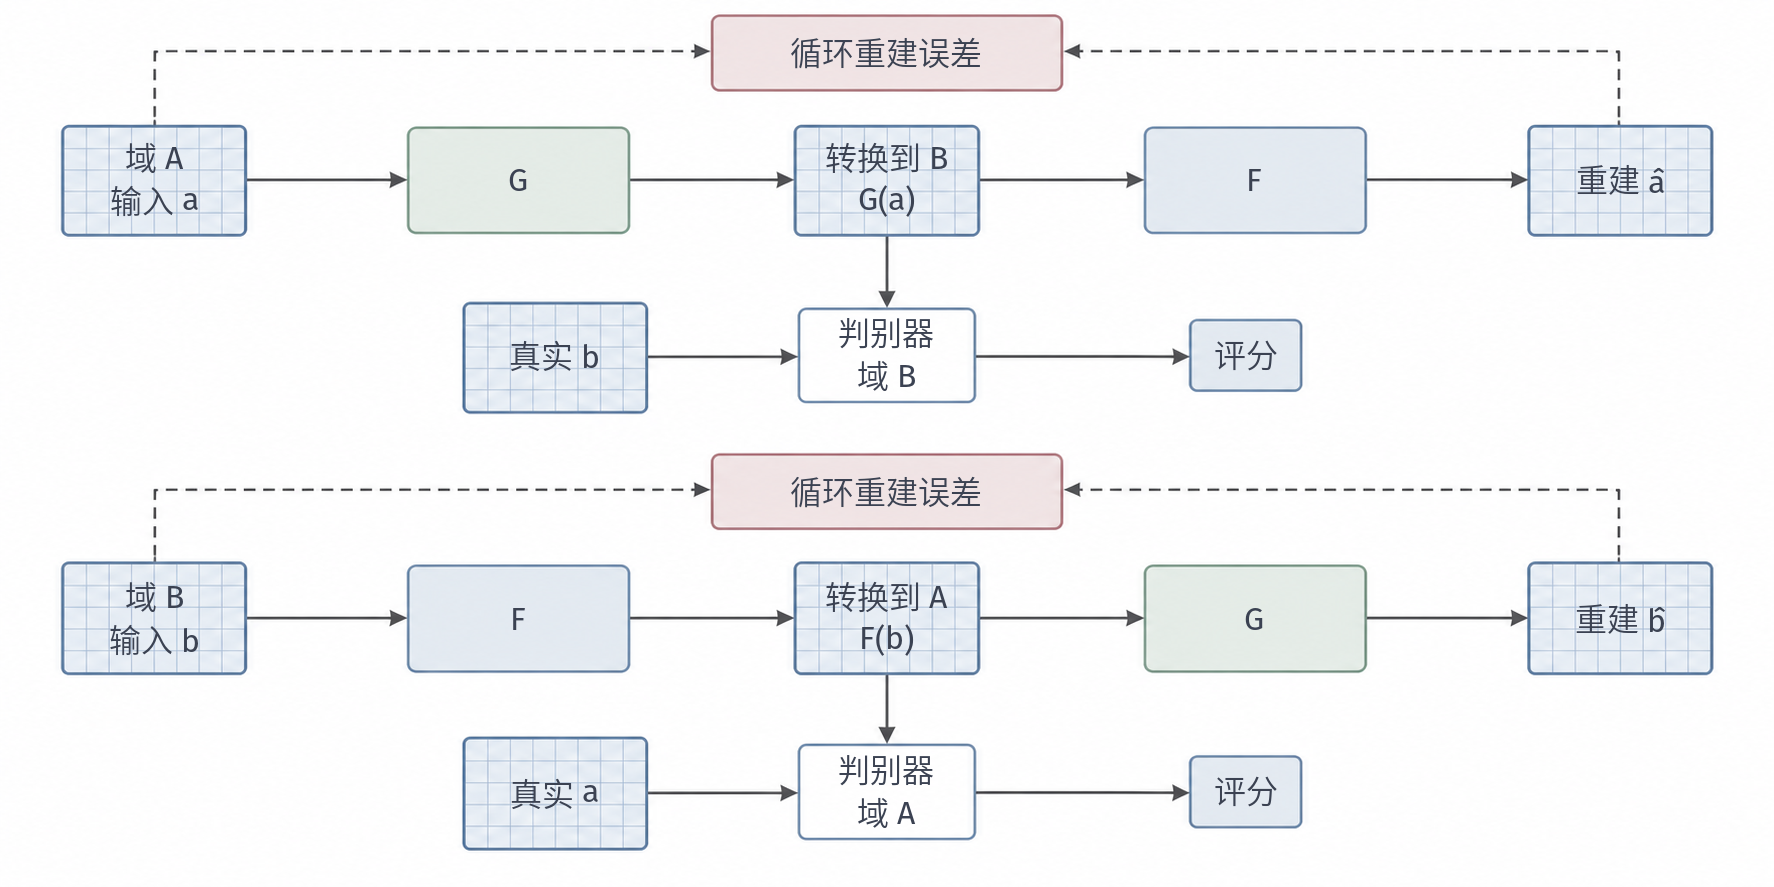
\includegraphics[width=156mm]{figures/08-neural-network-models/00-shared/generated/neural-generative-architectures/cyclegan/figure.png}
  \caption{CycleGAN的两条循环转换路径。$G$把域$\mathcal A$的输入转换到域$\mathcal B$，$F$执行反向转换；两个域的判别器分别比较真实样本与转换结果，虚线将原输入和重建结果送入循环重建误差。同名的$G$或$F$共享参数，$\bm a$与$\bm b$不要求配对。结构依据Zhu等（2017）。}
  \label{fig:neural-generative-cyclegan-structure}
\end{figure*}

两个方向分别比较起点与来回输出，循环重建误差为
\begin{equation}
  \label{eq:neural-generative-cycle}
  L_{\mathrm{cyc}}(G,F)
    =\mathbb{E}_{\bm{A}}\lVert F(G(\bm{A}))-\bm{A}\rVert_1
     +\mathbb{E}_{\bm{B}}\lVert G(F(\bm{B}))-\bm{B}\rVert_1.
\end{equation}
记$L_{\mathrm{adv}}(G,D_{\bm{B}})$为比较$G(\bm{A})$与真实$\bm{B}$的GAN对抗目标，反方向同理，则共同目标可写为
\[
  \begin{aligned}
  \min_{G,F}\max_{D_{\bm{A}},D_{\bm{B}}}\quad
      &L_{\mathrm{adv}}(G,D_{\bm{B}})
       +L_{\mathrm{adv}}(F,D_{\bm{A}})\\
      &+\lambda L_{\mathrm{cyc}}(G,F),\qquad\lambda>0.
  \end{aligned}
\]
对抗项规定转换后应属于哪个外观分布，循环项要求转换图仍包含足够信息，供另一网络恢复原输入。只做重建要求两转换器互相恢复，却没有约束中间图像是否符合目标域的真实外观；只做来源比较又不规定输入与输出的联系。两种约束需要共同使用。

训练时分别从两组图像抽样，不把同时抽到的两张图视为配对。固定$G,F$，两个判别器各自学习来源判断；固定判别器，更新两个转换器，循环误差的梯度经过$F\circ G$和$G\circ F$中的两网络。上式用原GAN的对数形式说明共同结构，CycleGAN原实现用平方误差：判别器把真实图输出向1拟合、把转换图输出向0拟合，生成器让转换图的判别输出接近1。原实现还用近期生成图像的缓冲区更新判别器，减弱其只跟随最新生成器输出的变化\scite{neural-generative-zhu2017}

训练需要同时保留两转换器与两判别器，并计算双向重建；在单个网络规模可比时，相对于只训练一个方向的配对转换，这些额外网络与路径增加了训练成本。使用时则只保留需要的方向，例如给出马照片$\bm{a}$，直接计算$G(\bm{a})$；标准CycleGAN不再为同一输入额外抽取随机向量，因此转换通常是确定性的。

即使两个方向的循环重建误差都为零，仍不能确定唯一的语义对应。假设两域各有两个等概率样本，分别表示站立与奔跑的动物。把站立对应到站立、奔跑对应到奔跑，再让$F$使用逆映射，可以完全匹配两域分布且重建为零；把这两个对应交换，并同时改变$F$，也满足同样条件。零重建误差排除了前面两输入合成一个结果的情形，却没有排除这些不同的双射。实际训练使用有限权重的循环惩罚，只是抑制导致重建误差的信息丢失，不能保证误差已经为零。因此，真实任务中“只增加条纹而保持姿态和背景”还依赖数据与网络结构，不能仅由循环目标推出。

pix2pix用真实配对目标直接约束当前输出，CycleGAN则用原输入约束来回输出，换取对无配对数据的适用性。这个替换引入了近似可逆的要求：需要删除输入信息，或从一个输入产生多种不同结果时，确定性双向转换可能不合适。CycleGAN所放宽的是训练数据的配对要求，并没有把所有受控生成任务都变成可解的无配对转换。

\section{基于风格控制的生成对抗网络}
\label{sec:neural-generative-stylegan}

条件生成需要训练样本告诉模型哪个标签或输入对应哪种输出。如果只有一批未标注的人脸照片，仍可能希望在生成后分别调整姿态、发型与细小纹理。这里没有可直接接入的属性条件，需要先改变生成器内部允许我们调节的位置，再检查这些位置实际控制了什么。

\subsection{网络结构}
\label{sec:neural-generative-stylegan-structure}

普通生成器把随机向量放在入口，由后续各层共同把它变成图像。这个结构可以产生多样图像，却有一个控制上的缺陷：入口的随机坐标与最终图像的可理解属性之间没有任何对应关系——你想只改发型、保留身份，但挪动某个$\bm z$坐标时，姿态、光照、发色往往一起变，因为这些因素在深层网络里早就纠缠在一起，无法分开调节。而前述逐级上采样的生成器已经沿不同尺度形成图像：小特征图组织较大范围的关系（姿态、脸型），之后的层再补充更细的空间变化（肤色、发丝）。这提示了一条思路：若不同尺度能够分别接收各自的调节量，便可能在不同层级分别控制“大结构”和“小细节”，而不是把所有变化都压在一个输入向量里。

Karras、Laine和Aila于2018年公开、2019年发表的StyleGAN，先在随机输入和合成网络之间加了一层可学习的“解耦”缓冲：把随机输入$\bm z$先经过映射网络$M$，得到一个中间向量$\bm{w}=M(\bm{z})$，再用$\bm{w}$控制合成网络的多个层。为什么要多此一举？因为标准高斯$\bm z$的各坐标必须相互独立、均匀地覆盖整个空间，无法贴合真实人脸那种“某些组合常见、某些组合根本不存在”的弯曲分布；经过$M$非线性变换后，$\bm{w}$所在空间的密度可以随数据自由塑形，把更多“容量”分配给真实存在的人脸组合。映射网络是共同训练的前馈网络；外部随机源仍便于采样，中间向量的分布则随$M$学习，不必在各坐标上照搬外部随机源的指定分布。这为合成网络学习适合图像变化的表示留下了自由，但不自动使每个坐标对应一个独立语义\scite{neural-generative-karras2019}

合成网络从一个可学习的低分辨率常量张量开始，再逐步提高分辨率。这个常量在不同样本之间共享，变化来自每层收到的调节量和噪声——这与以往“所有差异都来自输入向量”很不一样，输入向量$\bm w$在此更像是一组逐层下发的“风格指令”，而初始画布是固定的。每层有自己的仿射变换，从同一$\bm{w}$得到该层各通道的缩放与偏移；层的分辨率和通道数不同，得到的调节量也不同。随机输入由此可以在多个尺度直接参与计算，而不必只通过第一层的特征传播到全部后续位置。

那“风格指令”具体怎样作用于一层特征？原StyleGAN借用并改造了实例归一化：先把每个样本、每个通道在空间位置上的响应归一化到统一尺度，再用从$\bm w$算出的系数重新决定该通道该放大多少、平移多少——相当于先擦掉这一层原有的“浓淡”，再按风格指令重新上色。它先把一个样本内某个通道的空间响应归一化，再用风格给出的系数改变其尺度与偏移。对第$c$个特征通道$\bm{h}_c$，写为
\begin{equation}
  \label{eq:neural-generative-stylegan-adain}
  \operatorname{AdaIN}(\bm{h}_c,\bm{w})
    =s_c(\bm{w})\frac{\bm{h}_c-\mu_c}{\sigma_c}
      +b_c(\bm{w}),
\end{equation}
其中$\mu_c,\sigma_c$是当前通道在空间位置上的均值与标准差，实际计算对分母加入小常数；$s_c,b_c$由该层的仿射变换计算。所谓“风格”首先指这组通道调节量，而不是已经标明的发色、表情或姿态。每个系数作用于一个通道的全部空间位置，因此可以共同改变一类特征的响应。

人脸照片里还有一类变化与“风格”不同：单根头发的具体位置、皮肤毛孔、雀斑这些细节是近乎随机、逐像素变化的，让同一个全局的$\bm w$去编码每一根发丝既低效也无必要。StyleGAN因此区分两种随机源：有组织的外观交给各层风格，纯粹的局部偶然细节则交给逐空间位置独立的噪声图。StyleGAN为各层另行抽取独立的单通道高斯噪声图，图内不同空间位置独立变化；同一噪声图广播到该层各通道，再乘以可学习的通道系数后注入特征。风格系数在空间上共享（同一层所有位置共用一组缩放平移），噪声在空间上逐点变化，两者提供的是“整体风格”与“局部随机”两种不同的调节方式\scite{neural-generative-karras2019}

固定$\bm{w}$而重抽噪声，可以观察细小随机纹理怎样变化；固定噪声而改变不同层的风格，可以观察较有组织的外观变化。原论文在人脸任务中观察到较粗层影响姿态等大范围属性，较细层影响颜色和细节，但这些是训练后的经验分工。网络没有被约束为“每层只改变一种语义”。图~\ref{fig:neural-generative-stylegan-structure}可对照中间向量、逐层仿射变换与空间噪声的进入位置，看到分层调节如何沿逐级上采样传到最终图像。
\begin{figure*}[tbp]
  \centering
  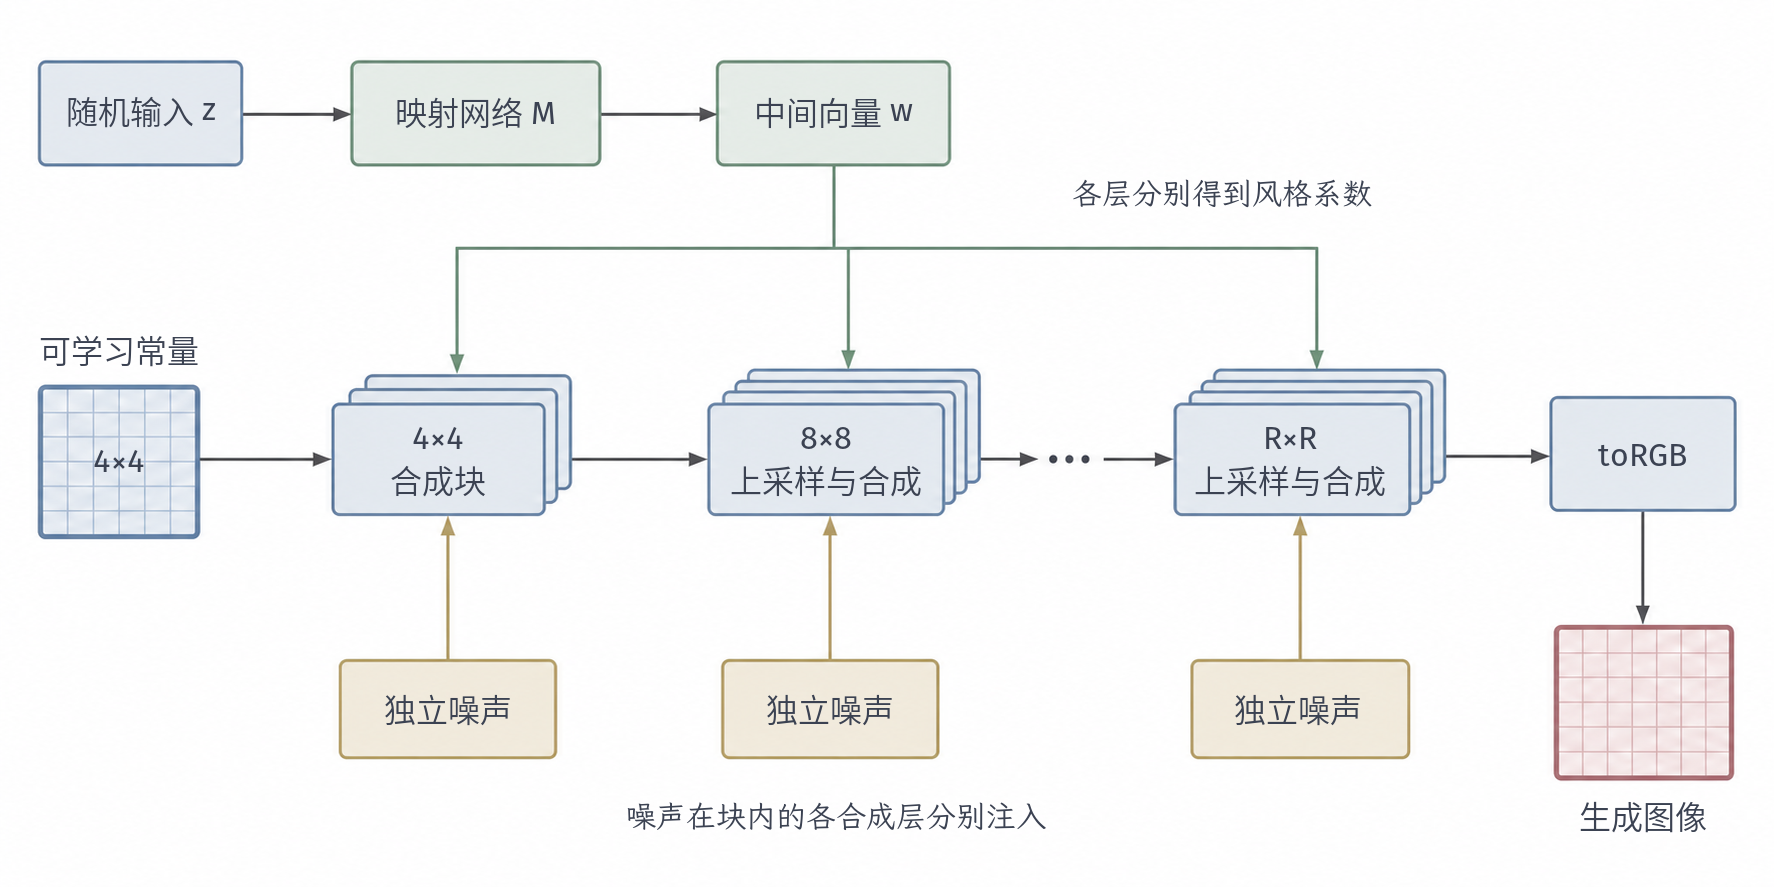
\includegraphics[width=156mm]{figures/08-neural-network-models/00-shared/generated/neural-generative-architectures/stylegan-overall/figure.png}
  \caption{StyleGAN系列的分层合成主干。随机输入经映射网络得到$\bm w$，各层据此计算自己的风格系数；可学习常量依次经过$4\times4$、$8\times8$及更高分辨率的合成块，到最终边长$R$的分辨率，其中$R$表示最终图像的空间边长；toRGB把特征通道映成彩色像素。每个噪声框表示块内各合成层分别使用的独立噪声，不表示整个块共用一个噪声。图中只保留特征主干与最终toRGB路径，省略中间RGB支路；StyleGAN2的默认结构还将各分辨率的toRGB结果逐级上采样并相加，toRGB也有自己的风格调制。块内差异见图\ref{fig:neural-generative-stylegan-blocks}。结构依据Karras等（2019，2020）。}
  \label{fig:neural-generative-stylegan-structure}
\end{figure*}

\subsection{参数学习与生成控制}
\label{sec:neural-generative-stylegan-learning}

StyleGAN仍用真实图像与生成图像的来源比较训练两方。生成损失回传到映射网络、共享常量、各层仿射变换、卷积核和噪声注入系数；抽取的噪声值是本次生成的输入，不是需要逐张记住的参数。与改变对抗评分的WGAN相比，StyleGAN主要改变生成器内部的表示与调节方式，二者的变化发生在不同位置。

训练通常会让同一个$\bm{w}$控制全部层，这也可能使相邻层依赖它们总能收到相同输入。为使分层交换可用，StyleGAN采用风格混合正则化：抽取两个随机输入，经$M$得到$\bm{w}_1,\bm{w}_2$，随机选择一个层间位置，在它之前使用$\bm{w}_1$，之后使用$\bm{w}_2$。网络于是需要学习处理来自不同样本的两组层级调节量，减弱对所有层风格共同变化的依赖。交换哪些层会产生哪些语义变化，仍需检查生成结果。

正常生成时，先抽取$\bm{z}$并计算$\bm{w}$，再算出各层风格、抽取各层噪声，最后运行合成网络得到图像，判别器不参与生成。若要比较不同尺度的风格对生成结果的影响，可以保留一张图的粗层风格，把细层风格换成另一张图的风格。这个操作提供了分层组合的入口，但不保证细层交换一定保留身份，也不保证任意组合都符合真实数据中的共现关系。

还可以把$\bm{w}$向映射后向量的均值$\overline{\bm{w}}$收缩，即使用$\overline{\bm{w}}+\psi(\bm{w}-\overline{\bm{w}})$，其中$0\leq\psi\leq1$，均值可用一批随机输入经$M$映射后估计。这个截断操作减少偏离均值的风格，可能减少部分极端输出，也会压缩生成变化并改变输出分布。即使风格完全收缩到均值，空间噪声仍可能产生差异；评价时应同时考察图像质量和变化覆盖，不能只看少量选出的结果。

\subsection{优化表达能力}
\label{sec:neural-generative-stylegan-expression-extension}

逐样本归一化虽然提供了直接调节通道的方法，也可能抹去通道之间原有的幅度关系。假设某通道只有一个位置出现很高的响应，这个局部峰值就会改变整个通道的均值与标准差，使其他位置同时受到归一化影响。StyleGAN2论文在原模型的中间特征与生成图像中分析了类似水滴的斑点，并提出局部高响应可能被用来绕过归一化对信号幅度的限制。这是其结构改动的依据，而不是对所有生成伪影的统一解释\scite{neural-generative-karras2020}

Karras、Laine、Aittala等于2019年公开、2020年发表StyleGAN2，保留中间向量与逐层风格输入，改变风格对卷积的作用方式。先用风格缩放各输入通道对应的卷积权重，再根据调制后权重的尺度进行解调制。这样仍能改变各输入通道的相对贡献，却不再读取当前特征图的空间均值与方差来归一化整张特征图。

记卷积核为$w_{o,c,u,v}$，$o,c$分别是输出与输入通道，$u,v$是核内坐标；风格给出输入通道系数$s_c$。调制后的权重为$w'_{o,c,u,v}=s_cw_{o,c,u,v}$。若用输入各项不相关且方差为1的近似估计输出尺度，某输出通道的方差就是对应权重平方的和。因此，对每个输出通道使用
\begin{equation}
  \label{eq:neural-generative-stylegan-demodulation}
  w''_{o,c,u,v}
    =\frac{s_cw_{o,c,u,v}}
      {\sqrt{\sum_{c,u,v}(s_cw_{o,c,u,v})^2+\epsilon}},
      \qquad\epsilon>0.
\end{equation}
其中小常数$\epsilon$避免分母为零。解调制控制的是权重所预计的输出尺度，不保证实际特征彼此独立，也不保证实际输出方差严格为1。偏置与空间噪声在调制卷积之外加入，使它们的作用不再被同一逐样本归一化消除。

图~\ref{fig:neural-generative-stylegan-blocks}在首个$4\times4$合成块上对照两种计算。原模型通过AdaIN直接归一化特征，StyleGAN2则把风格作用放入卷积权重，并将噪声加在调制卷积之后。整体的映射网络与分层输入仍然保留，替换的是合成层内部怎样使用风格与噪声。
\begin{figure*}[tbp]
  \centering
  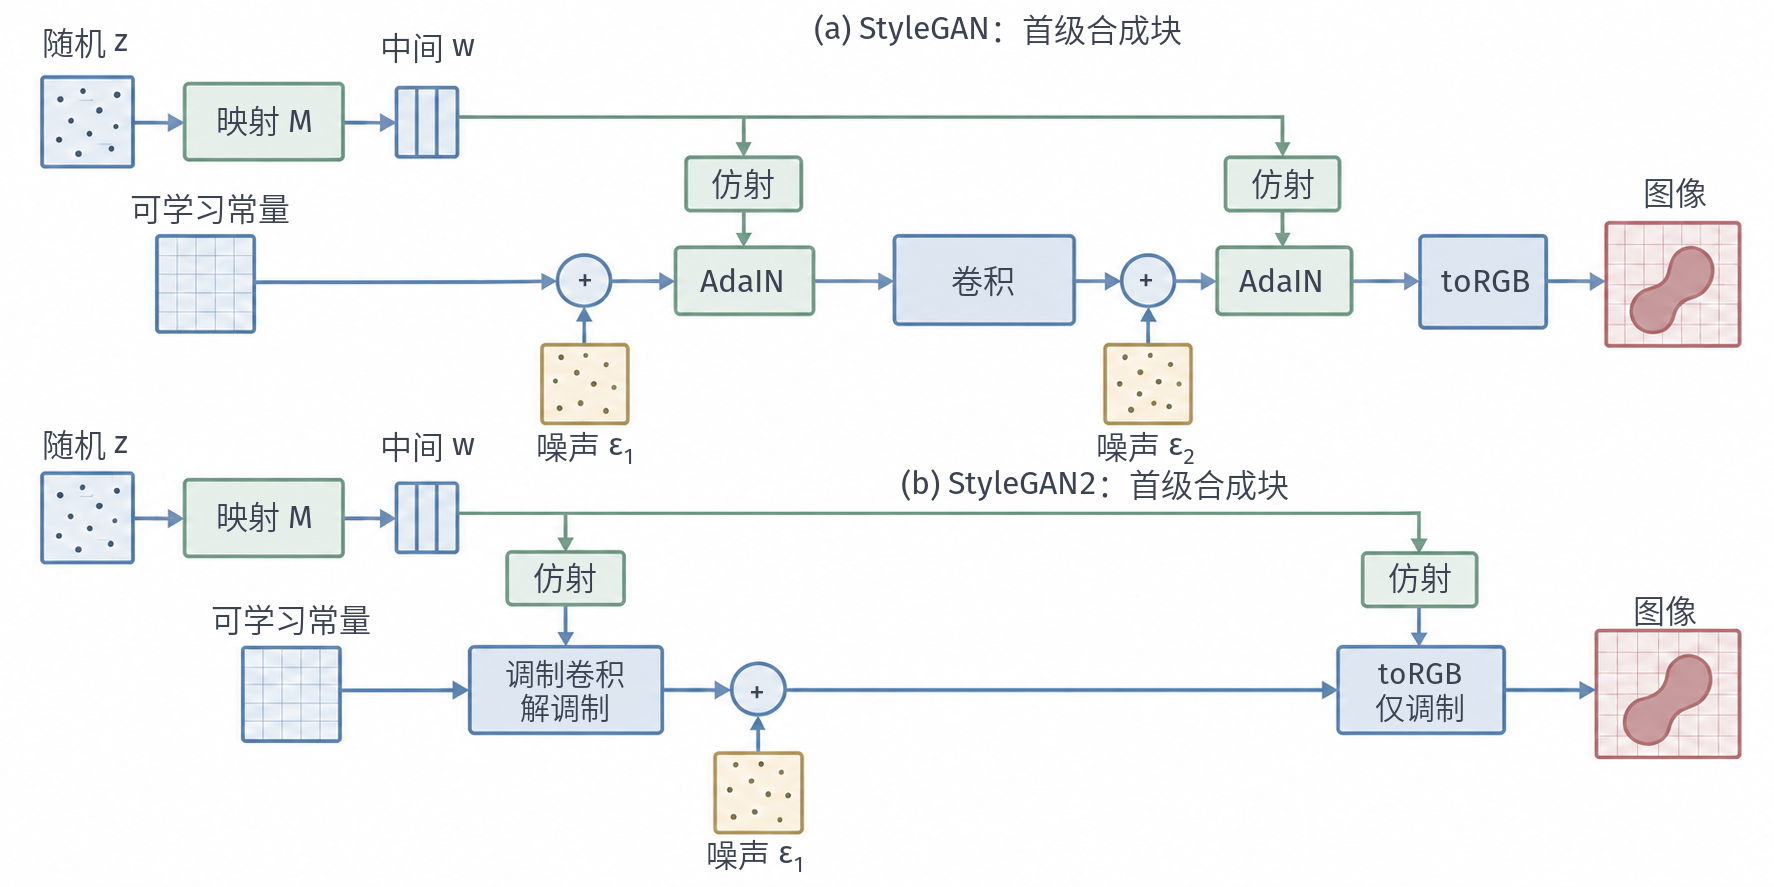
\includegraphics[width=156mm]{figures/08-neural-network-models/00-shared/generated/neural-generative-architectures/stylegan/figure.png}
  \caption{StyleGAN与StyleGAN2首个$4\times4$合成块的对照。两者都从可学习常量出发，并由映射向量分别生成风格系数；原StyleGAN在常量和卷积输出处加入噪声，再用AdaIN调节特征。StyleGAN2首级只有一层调制与解调制卷积，在卷积输出处加入噪声，toRGB使用调制而不使用解调制。两面板仅展示首级产生的RGB支路，省略偏置、激活及后续分辨率层；整体路径见图\ref{fig:neural-generative-stylegan-structure}。结构依据Karras等（2019，2020）。}
  \label{fig:neural-generative-stylegan-blocks}
\end{figure*}
\FloatBarrier
StyleGAN2还处理了中间向量改变时输出变化过于不均的问题。同样大小的中间向量改动，在某些位置可能几乎不改变图像，在另一些位置却可能引起很大的像素变化。要约束这种敏感度，需要先把中间向量的改动与生成图像的局部响应联系起来。

固定本次各层的空间噪声，将这些噪声输入合记为$\bm{\eta}$，把图像的全部像素展平。若中间向量的维数为$d_w$，合成映射可写为$g_{\bm{\eta}}:\mathbb{R}^{d_w}\to\mathbb{R}^{d}$。在关于$\bm{w}$可微的位置，记其Jacobian矩阵为$\bm{J}_{\bm{w}}\in\mathbb{R}^{d\times d_w}$；它也依赖本次固定的噪声。足够小的$\Delta\bm{w}$引起的图像变化满足
\begin{equation}
  \label{eq:neural-generative-stylegan-local-response}
  g_{\bm{\eta}}(\bm{w}+\Delta\bm{w})-g_{\bm{\eta}}(\bm{w})
    =\bm{J}_{\bm{w}}\Delta\bm{w}
       +o(\lVert\Delta\bm{w}\rVert_2).
\end{equation}
因此，$\bm{J}_{\bm{w}}$描述当前中间向量附近，哪些方向的改动会怎样传到图像。高分辨率图像包含大量像素，直接保存整个矩阵会增加计算与存储；训练可以先把像素随机加权成一个标量，再通过这个标量的梯度检查局部响应。

路径长度正则化先为输出像素抽取高斯随机系数。为说明基本关系，令$\bm{y}\sim\mathcal{N}(\bm{0},\bm{I}_d)$，每个坐标为对应像素提供一个随机权重，再把生成图像按这些系数加权成标量$\langle g_{\bm{\eta}}(\bm{w}),\bm{y}\rangle$。固定这次抽到的$\bm{y}$，链式法则给出
\begin{equation}
  \label{eq:neural-generative-stylegan-projected-gradient}
  \nabla_{\bm{w}}\langle g_{\bm{\eta}}(\bm{w}),\bm{y}\rangle
     =\bm{J}_{\bm{w}}^{\top}\bm{y}.
\end{equation}
对这个标量做一次反向求导，就能得到同一Jacobian的反向随机投影，无须显式构造整个矩阵。换一个中间向量、空间噪声或像素权重，就检查另一处或另一种投影。投影梯度的长度由生成映射的局部响应决定，因此可以用来约束前面所说的变化敏感度；它本身并不是一次前向改动产生的图像距离。

记训练中持续估计的平均梯度长度为$a_{\mathrm{pl}}$，以共享一个$\bm{w}$的上述写法，惩罚项可表示为
\begin{equation}
  \label{eq:neural-generative-stylegan-path-regularization}
  R_{\mathrm{pl}}
    =\mathbb{E}_{\bm{w},\bm{\eta},\bm{y}}
       \bigl(\lVert\bm{J}_{\bm{w}}^{\top}\bm{y}\rVert_2
               -a_{\mathrm{pl}}\bigr)^2.
\end{equation}
这里$\bm{w}$由随机输入经映射网络得到，空间噪声和像素权重与它独立抽取。先计算当前小批量的梯度长度均值，再用指数移动平均更新$a_{\mathrm{pl}}$：保留一部分此前的平均值，加入一部分当前均值。具体地，令$t$表示第$t$次计算这项正则化，$\overline{\ell}^{(t)}$是该批次的梯度长度均值，选择$0<\beta_{\mathrm{pl}}<1$，从给定初值开始更新
\[
  a_{\mathrm{pl}}^{(t)}
    =\beta_{\mathrm{pl}}a_{\mathrm{pl}}^{(t-1)}
       +(1-\beta_{\mathrm{pl}})\overline{\ell}^{(t)}.
\]
反复代入这条更新后，越早的批次乘上的$\beta_{\mathrm{pl}}$越多，权重逐次衰减；新批次因而可以持续调整目标尺度。这个平均值是随训练维护的统计量，不是另一个用梯度下降学习的网络参数。平方惩罚将梯度长度拉向这个动态平均，鼓励不同$\bm{w}$和不同随机系数下的响应幅度接近。实际实现还可按合成层分别统计，并按图像尺寸缩放随机像素系数；这里的简式用于说明随机投影与惩罚的共同结构。

这项约束检查的是合成图像相对于中间向量的局部响应；WGAN-GP检查的则是评价器相对于图像输入的梯度，两者的求导对象不同。这里调整的是变化尺度，没有把梯度指定为发色或姿态等语义，有限随机投影的软惩罚也不保证所有位置和方向严格等距。计算这项约束时，还需把包含梯度长度的惩罚回传到生成网络参数，因而增加求导成本；原实现采用间隔若干步再计算的方式控制额外开销\scite{neural-generative-karras2020}

原StyleGAN沿用了渐进增长来组织高分辨率训练，StyleGAN2又检查了随训练增加网络阶段的影响。其多分辨率合成结构可以保留固定网络拓扑，将不同分辨率特征转成图像贡献，再把低分辨率贡献上采样后与高分辨率贡献相加。它改变高分辨率细节参与合成的方式，与用权重解调制减少归一化伪影、用路径长度约束平衡变化敏感度，是同一生成任务中的不同改动。

StyleGAN2仍从随机输入生成图像，也仍用对抗训练；它针对原StyleGAN的伪影与变化控制作结构和训练改进，没有增加一个新的输出任务。StyleGAN与cGAN则提供两种不同控制依据：cGAN让训练样本已有的标签或输入规定要求，StyleGAN提供无标签的分层调节位置。两种结构可以组合，但要把某个风格方向解释成确定的语义属性，仍需额外的数据、分析或监督依据。

\section{模型关系与比较}
\label{sec:neural-generative-comparison}

这些模型都借助另一个网络获得生成学习信号，但改变的对象并不相同。把它们放回同一个任务，我们可以分别考察：图像怎样从输入形成，什么差异会进入训练目标，训练集提供哪些对应信息，以及生成时允许控制什么。区分这些问题，才能判断两种设计是在同一位置作替代，还是可以放进同一个模型。

\subsection{图像表示与分布比较}

GAN给出生成器和判别器相互学习的基本方式，DCGAN把两方具体组织成卷积网络。假设任务仍是从随机输入产生人脸：将全连接生成器换成逐级上采样的卷积生成器，会改变图像的构造与参数共享；训练中仍可使用来源分类与非饱和生成损失。这个变化主要利用图像中的空间规律，不能仅凭采用了卷积就认定生成分布已经覆盖全部人脸变化。

WGAN在另一位置改变设计。即使保留同一个卷积生成器，也可以把来源判别器换成受变化幅度约束的实值评价器，再按两组评分差训练。因而“使用DCGAN式卷积骨架”与“使用WGAN式比较目标”可以同时成立。前者回答如何表示图像，后者回答什么差异能形成学习信号。替换目标时还须相应改变评价器末层、约束和更新方式，不能只把对数损失的名称换掉。

WGAN-GP保留实值评分目标，用抽样梯度惩罚替代权重裁剪，针对的是评价器约束过于粗糙的问题。它增加了输入梯度的计算，也需要避免评价器把不同样本通过批量归一化耦合起来。渐进式增长则沿训练阶段改变生成与判别的分辨率。这些方法可以改善不同环节的训练条件，但最终图像的合理性、变化范围和训练成本仍须分别检查。

\subsection{条件信息与监督约束}

无条件GAN拟合所有观测的总体变化，条件GAN把任务分解到已知类别或属性之下。例如，指定数字“3”后，生成器仍须产生不同写法；条件判别器要检查这些写法与“3”是否相容。这个设计增加了生成时可给定的信息，却没有提供某个随机输入应该对应哪一张真实图的像素答案。

pix2pix的图像条件带有更强的监督：训练集把每张输入与目标图配在一起。生成器既接受目标域纹理的判别，又接受当前样本的配对重建约束。U-Net跳接让输入中的位置细节进入解码，PatchGAN把学习信号细化到局部图像块；两者分别处理内容传递与局部外观。若训练集只有彼此独立的两组图，pix2pix的配对误差就没有可据以计算的目标，不能把任意两张图配在一起沿用它。

CycleGAN用两个方向的转换和循环重建补上无配对条件下的信息保持要求。它比只匹配目标域增加了“来回后能恢复输入”的约束，却仍没有给出哪张马图应对应哪张斑马图的真实答案。pix2pix和CycleGAN因此是在不同监督条件下解决转换问题：前者利用已知对应，后者在没有对应时引入近似可逆的限制。把后者用于一张轮廓可以对应许多照片的任务时，还要检查循环要求是否压缩了应有的多种输出。

\subsection{随机变化与生成控制}

DCGAN主要在入口接收随机向量，StyleGAN则先得到中间向量，再在多个合成尺度施加风格调节。若要观察轮廓变化与细纹理变化的区别，分层调节提供了不同的操作位置，独立噪声另用于局部随机细节。它增加了组织和操纵生成变化的手段，没有直接把“表情”“发色”等语义标签变成受监督输入；需要这样的标签控制时，仍可考虑把条件信息加入训练。

StyleGAN2针对原StyleGAN特征归一化带来的问题，改为卷积核调制与解调制。两者保留映射网络和分层控制的总体思路，区别落在风格系数怎样作用于特征计算。渐进式增长与这种分层控制也不能混为一谈：前者安排训练时何时接入更高分辨率，后者安排生成时不同输入从哪些层进入。原StyleGAN采用过渐进训练，StyleGAN2的最终配置则从开始就保留各分辨率的层，把多尺度图像贡献相加，并在判别器中采用残差连接，以固定网络结构组织高分辨率学习。

例如，把姿态固定而只改变头发细节，类别条件、层间风格交换和随机噪声会给出不同操作。条件要求生成结果符合已知描述；风格交换把一组层的调节量替换成另一组；噪声变化则在已有组织之上改变局部随机细节。应根据希望保留的信息和允许改变的因素选择操作，再用生成结果检查实际影响范围。一个层级能被单独调节，不意味着它已经与某个人工语义严格对应。

\section{本章小结}
\label{sec:neural-generative-summary}

本章围绕章首提出的两条标准——单张样本要合理、整组样本要覆盖真实变化——组织了一条“生成器＋评判者”的技术路线。神经网络生成模型用输入变化和可学习映射产生新的观测：随机输入提供多种输出的来源，生成器决定这些输入怎样分配到观测空间；由于没有逐像素的标准答案，训练时借助另一个网络来判断生成结果与真实数据的分布差异。GAN通过来源判别学习这套比较，训练时两方像造假者与鉴画师一样交替更新、共同提高，使用时则只保留生成器；隐式采样模型不需要、通常也无法直接写出图像密度。

本章的方法从不同位置改进这套过程。卷积与分层合成组织图像表示，实值评分与梯度约束改变比较信号，条件和配对信息规定要生成什么，循环重建规定应保留哪些输入信息。结构图可以帮助追踪这些变化，但判断模型是否适合任务，还需同时查看训练数据、损失项以及生成时实际使用的路径。图像是否清晰、生成变化是否覆盖真实数据、给定条件或分层操作是否产生预期影响，是需要分别评价的问题；评价使用的真实样本应与训练数据分开。

\paragraph{延展阅读}
第\ref{sec:neural-generative-gan}节所引Goodfellow等的原始GAN论文，可结合两网络目标和梯度更新阅读；第\ref{sec:neural-generative-dcgan}节的DCGAN论文进一步说明卷积、激活和归一化怎样配合。若关注训练信号，可对照第\ref{sec:neural-generative-wgan}节的WGAN与WGAN-GP论文，区分分布比较与约束实现。条件生成和图像转换的监督差异见第\ref{sec:neural-generative-conditional}节所引条件GAN、pix2pix和CycleGAN论文；第\ref{sec:neural-generative-stylegan}节的StyleGAN与StyleGAN2论文则可用于比较特征归一化和核调制的生成控制。显式似然、潜变量推断及扩散生成的另一组机制，可沿章首给出的卷六“概率生成模型”章入口继续阅读。
